\begin{savequote}[8cm]
It's simple mathematics.
  \qauthor{--- Mos Def, "Mathematics"}
\end{savequote}

\chapter{\label{ch:3-methods}Theory and Methodology}

\minitoc

%% Books:

% For a really nice explanation of solid state QM basics - bloch waves, an electron in a crystal potential etc, see Lundstrom "fundamentals of carrier transport"

\section{Introduction} 

In this chapter I present the theory and methodology that underlies the work in this thesis. The chapter starts with an introduction to Density Functional Theory - first I introduce the theoretical concepts, then I provide details about how DFT is implemented in practice. In the second part of the chapter I outline how we can use DFT energies combined with a number of post-processing steps to predict defect formation energies and charge transition levels. The chapter ends with an introduction to the theory of lattice dynamics and how this is used to calculate the vibrational properties of a material. 

\section{Density Functional Theory} \label{DFTtheory}

Density Functional Theory is the most commonly used method of electronic structure calculation in condensed matter physics and quantum chemistry. 
Using DFT we are able to predict the ground state properties of a material including electron density, total energy, equilibrium structure, vibrational frequencies and properties relating to the difference in total energies, such as defect formation energies or surface energies. 
As DFT is a ground state theory, we are not able to calculate properties relating to to excited states and, without further calculations (such as those outlined in Section \ref{sec:latticedynamics}), results do not incorporate the effects of temperature. 

The theoretical basis for DFT was established in 1964 through the work of Walter Kohn and Pierre Hohenberg.\autocite{Hohenberg1964} This was further developed by Walter Kohn and Lu Jeu Sham to produce Kohn-Sham DFT.\autocite{Kohn1965} However it was not until the late 1980's that work started on building approximations to the exchange-correlation functional so that DFT could be used in practice. 

There are a growing number of codes that implement DFT, many of which include extensions to DFT so that excited state properties can be predicted.
Although some codes aspire to a blackbox approach, with the user protected from the underlying mechanics of DFT, for most systems of interest an understanding of the underlying approximations and parameters used are required for reliable results.

\subsection{DFT in theory} %expand to include more equations, including slater determinant? and E\phi=H\phi.

Firstly, a note on the name. A function accepts one or more numbers as input and produces a number as output. Likewise, a functional accepts one or more \textit{functions} as inputs, and produces a number as output. In DFT the functional is the electron density which is a function of space and time.

Throughout this chapter, unless stated otherwise, we use the Born-Oppenheimer approximation: the heavy atomic nuclei are treated as fixed points, and we solve the ground state quantum mechanical problem for the electrons only. This reduces the number of degrees of freedom of the system, a tactic that will be used again later in the chapter.

Although no one single text is followed, concepts for the underlying theory have been taken from References \cite{Burke2007}, \cite{Scuseria05} and \cite{Perdew2010}.


\subsubsection{The Schr\"{o}dinger equation}

The Schr\"{o}dinger equation describes the wavefunction $\Psi$ of a quantum mechanical system. The wavefunction is a fundamental postulate of quantum mechanics and it contains all the information for a given system. Once the Schr\"{o}dinger equation is solved, and a wavefunction is found, all the physical properties for that system follow. To take the simplest possible example, the time-independent non-relativistic Schr\"{o}dinger equation for a single particle can be written as:
\begin{equation} \label{singleparticle}
\left[\frac{-\hbar^2}{2m}\nabla^2+V(\textbf{r})\right]\Psi(\textbf{r}) = E\Psi(\textbf{r})
\end{equation}
where the first term in the bracket corresponds to the kinetic energy and the second term corresponds to the potential energy. For a single particle in a simple potential, such as the ``particle in a box" system or hydrogen atom, the Schr\"{o}dinger equation can be solved exactly. Unfortunately it is not possible to solve the Schr\"{o}dinger equation exactly for more complex systems, where there are multiple electrons interacting with each other (N-body or many-body systems). In this case, the Schr\"{o}dinger equation takes the form:
\begin{equation}
\left[\frac{-\hbar^2}{2m}\sum_{i=1}^N\nabla_i^2+\sum_{i=1}^Nv_{\textrm{ext}}(\textbf{r}_i)+\sum_{i<j}^N\frac{q_iq_j}{\lvert\textbf{r}_i-\textbf{r}_j\rvert}\right]\Psi(\textbf{r}_i) = E\Psi(\textbf{r}_i),
\end{equation}
where the third term in the square bracket describes the electrostatic interaction between two particles of charges $q_i$ and $q_j$, and couples the coordinates of the particles together.

The following methods (Hartree-Fock and Kohn-Sham DFT) give a way to obtain an approximate solution to the Schr\"{o}dinger equation for systems of interest. They do this by mapping the interacting problem onto a non-interacting problem with an effective potential $V_\textrm{s}(\textbf{r})$. In doing so, the dimensionality of the problem is greatly reduced. Instead of solving one N-dimensional probelem, which is computationally intractable, N one-dimensional problems are solved (Figure \ref{decouple}). These provide a compromise between accuracy and computational efficiency.

\begin{figure}[h]
\centering
  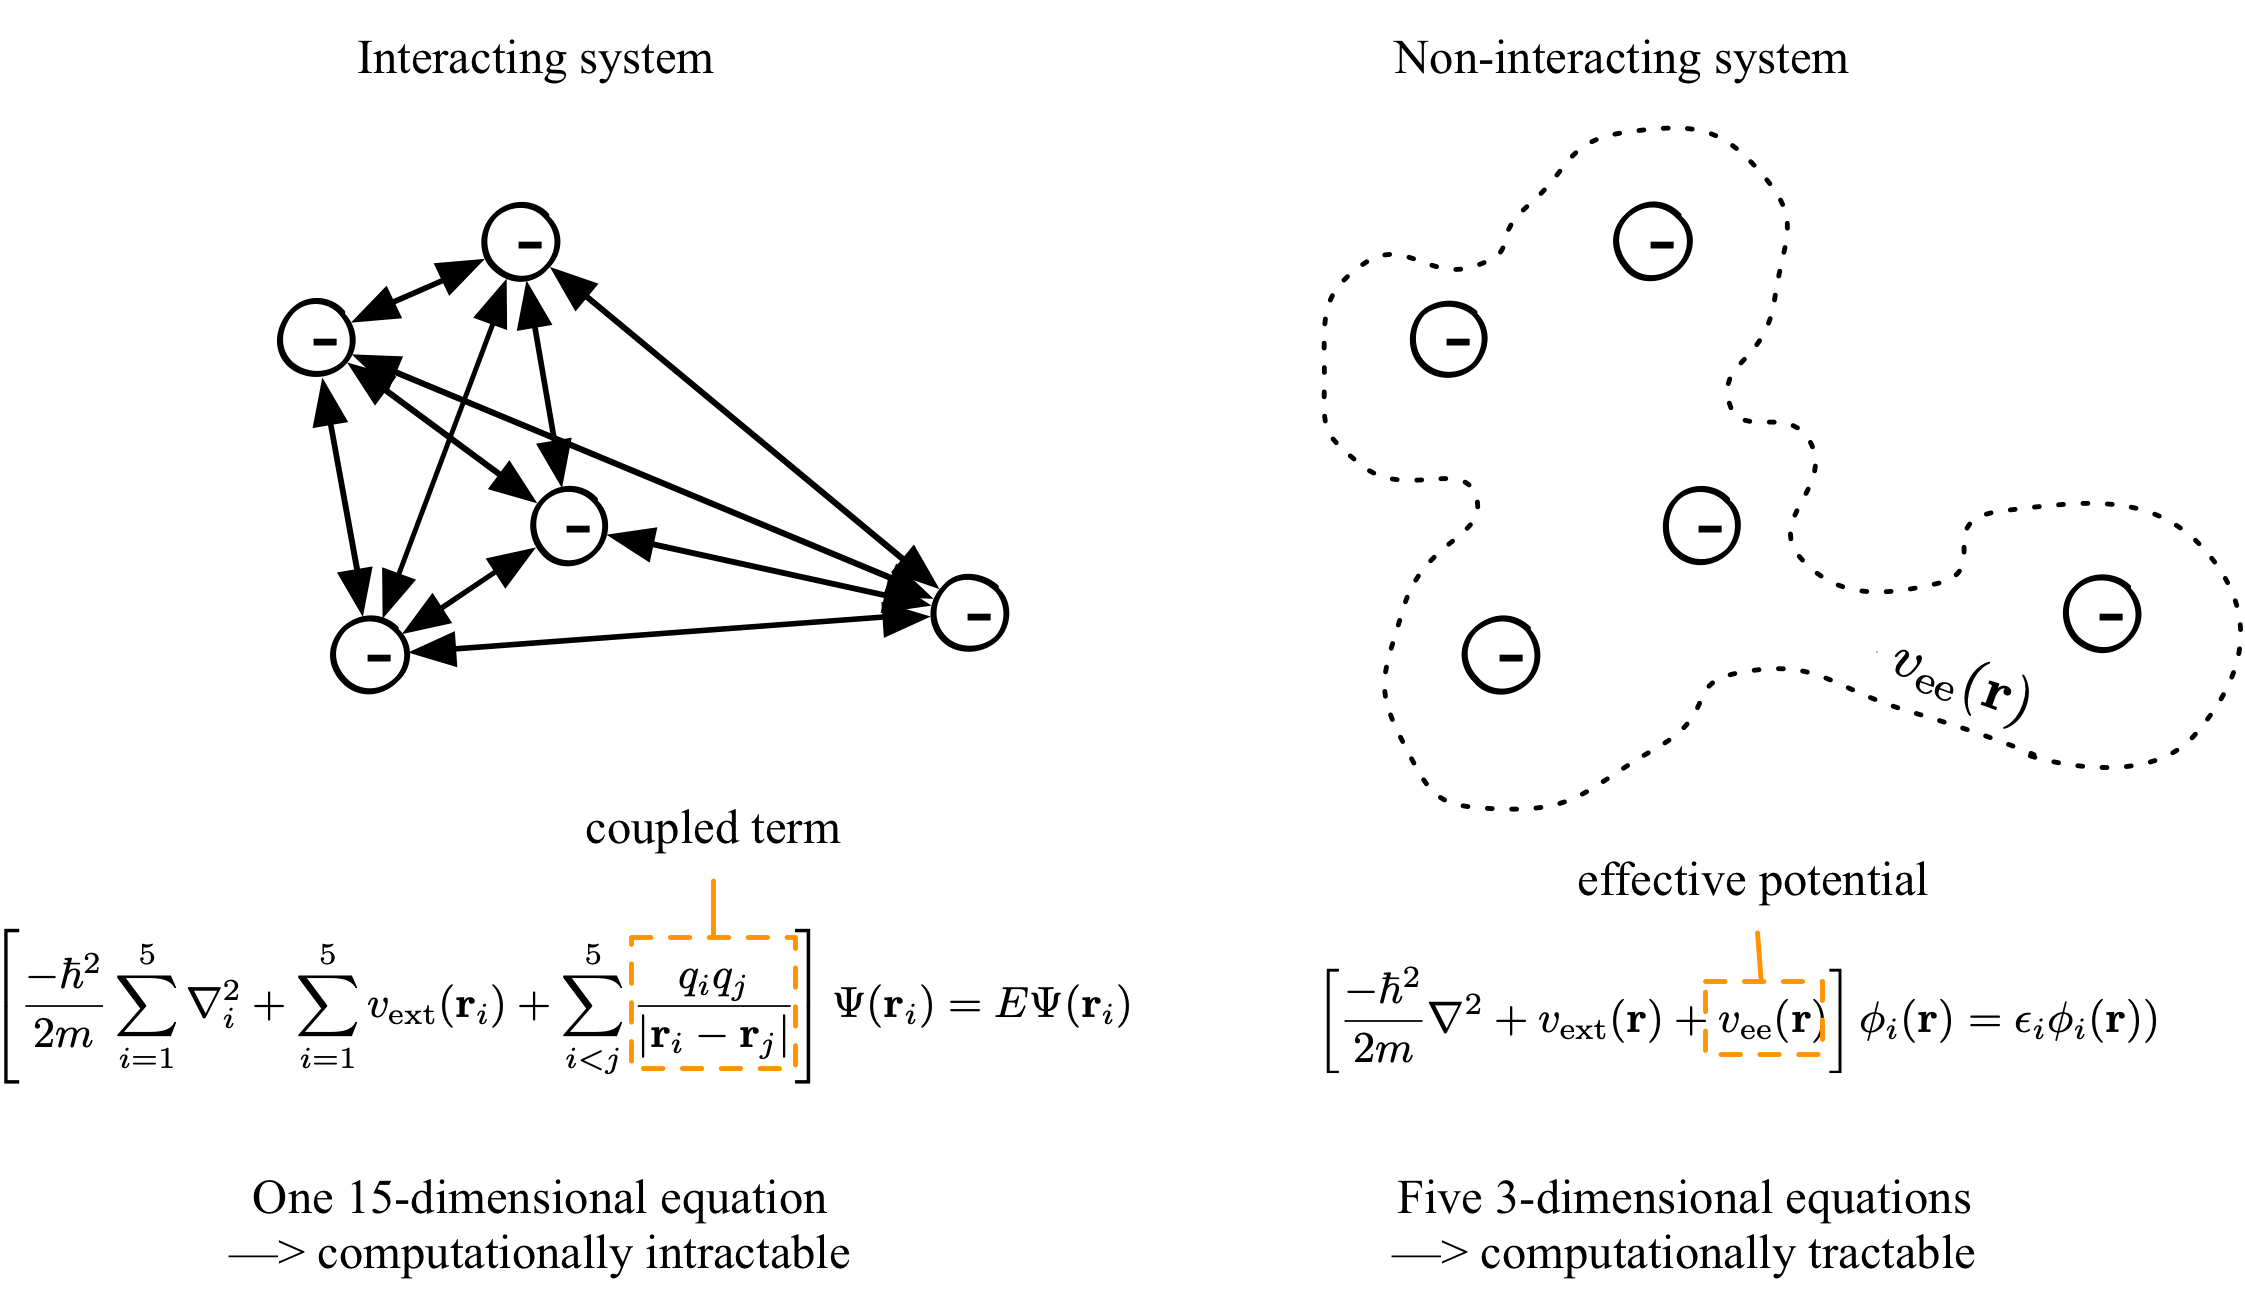
\includegraphics[width=1.0\columnwidth]{figures/ch3/decouple.png}
  \caption[Schematic outlining the equivalence between interacting and non-interacting systems]{Schematic outlining the equivalence between a system of interacting particles and a system of non-interacting particles in an effective potential. The underlying idea is that an interaction can be replaced by the equivalent potential. This maps the interacting 3N-dimensional problem onto N 3-dimensional problems. A consequence of this mapping is that the effective potential depends on the electron density which is itself dependant on the effective potential - a self-consistent set of equations is formed.} %update so q1q2 in couple term in picture
  \label{decouple}
\end{figure}

\subsubsection{Hartree-Fock methods}

Hartree-Fock methods introduced the concept of fictitious one-electron orbitals $\phi$ that do not interact with each other as a way of solving the Schr\"{o}dinger equation. The HF many-body wavefunction is a Slater determinant of the one-electron orbitals and is denoted with $\Phi$. 

The effective potential, introduced in Figure \ref{decouple}, is given by $V_{\textrm{ee}} = U + E_{\textrm{x}}$. $U$ accounts for the electrostatic interaction between electrons. Hartree-Fock methods model the charge interaction as a coulomb potential for a system of fixed electrons; the electrons feel the average electrostatic field due to the other electrons.

The second way electrons interact with each other is via their spin:
\begin{displayquote}
    Two MCs can't occupy the same space at the same time,
    it's against the laws of physics \\ \hspace{2cm}---Lauryn Hill, \textit{Zealots}
\end{displayquote}
Electrons with the same spin are indistinguishable, and a consequence of this is that the many body  wavefunction must be anti-symmetric. This leads to the Pauli Exclusion Principle, whereby two identical electrons (ie, electrons with the same spin and momentum) cannot occupy the same space at the same time. Hartree Fock methods account for electron exchange, the repulsion between electrons with parallel spins, exactly. 

Hartree-Fock methods do not give an exact solution to the Schr\"{o}dinger equation as they ignore electron correlation. This is the correlated motion of electrons with anti-parallel spins as a result of their mutual coulombic repulsion. It is a consequence of the fact that the true many body wavefunction is not formed from a simple Slater determinant.
% from http://newton.ex.ac.uk/research/qsystems/people/coomer/dft_intro.html

\subsubsection{The Hohenberg-Kohn theorems}

The 1964 Hohenberg-Kohn paper contains two key results: (i) the ground state electron density uniquely determines the ground state electronic wave function and, following this, all properties of the system; (ii) the true density functional for the electronic energy assumes its minimum for the correct ground-state density. % quote this from? http://publish.uwo.ca/~vstarove/PDF/tacc_chapter24.pdf

In Hartree-Fock methods, the potentials (external, coulomb and exchange) determine the properties of a system. First, Hohenberg and Kohn demonstrate that the density can be used instead to uniquely characterise the system; rather than solving the Schr\"{o}dinger equation for the wavefunction, we can solve it for the electron density. The energy can be expressed as
$$E\left[\rho\right]=\int v_{\textrm{ext}}(\textbf{r})\rho(\textbf{r})d\textbf{r}+T\left[\rho\right]+J\left[\rho\right]+E_{\textrm{xc}}\left[\rho\right].$$
For a fixed number of electrons the functional $F\left[\rho\right]=T\left[\rho\right]+J\left[\rho\right]+E_{\textrm{xc}}\left[\rho\right]$ is universal, and the only thing that varies between systems is the external potential (determined by the electron-nuclei interaction). 

Secondly, Hohenberg and Kohn show that the ground state energy can be found variationally; the density that minimises the total energy is the true ground state density.

This formalism has the advantage that the electron density has a lower dimensionality than the N-electron wavefunction (Figure \ref{}). The problem is that although the Hohenberg-Kohn theorem tells us that the terms $T\left[\rho\right]$ and $E_{\textrm{xc}}\left[\rho\right]$ exist, they are unknown and must be approximated.

\begin{figure}[h]
\centering
  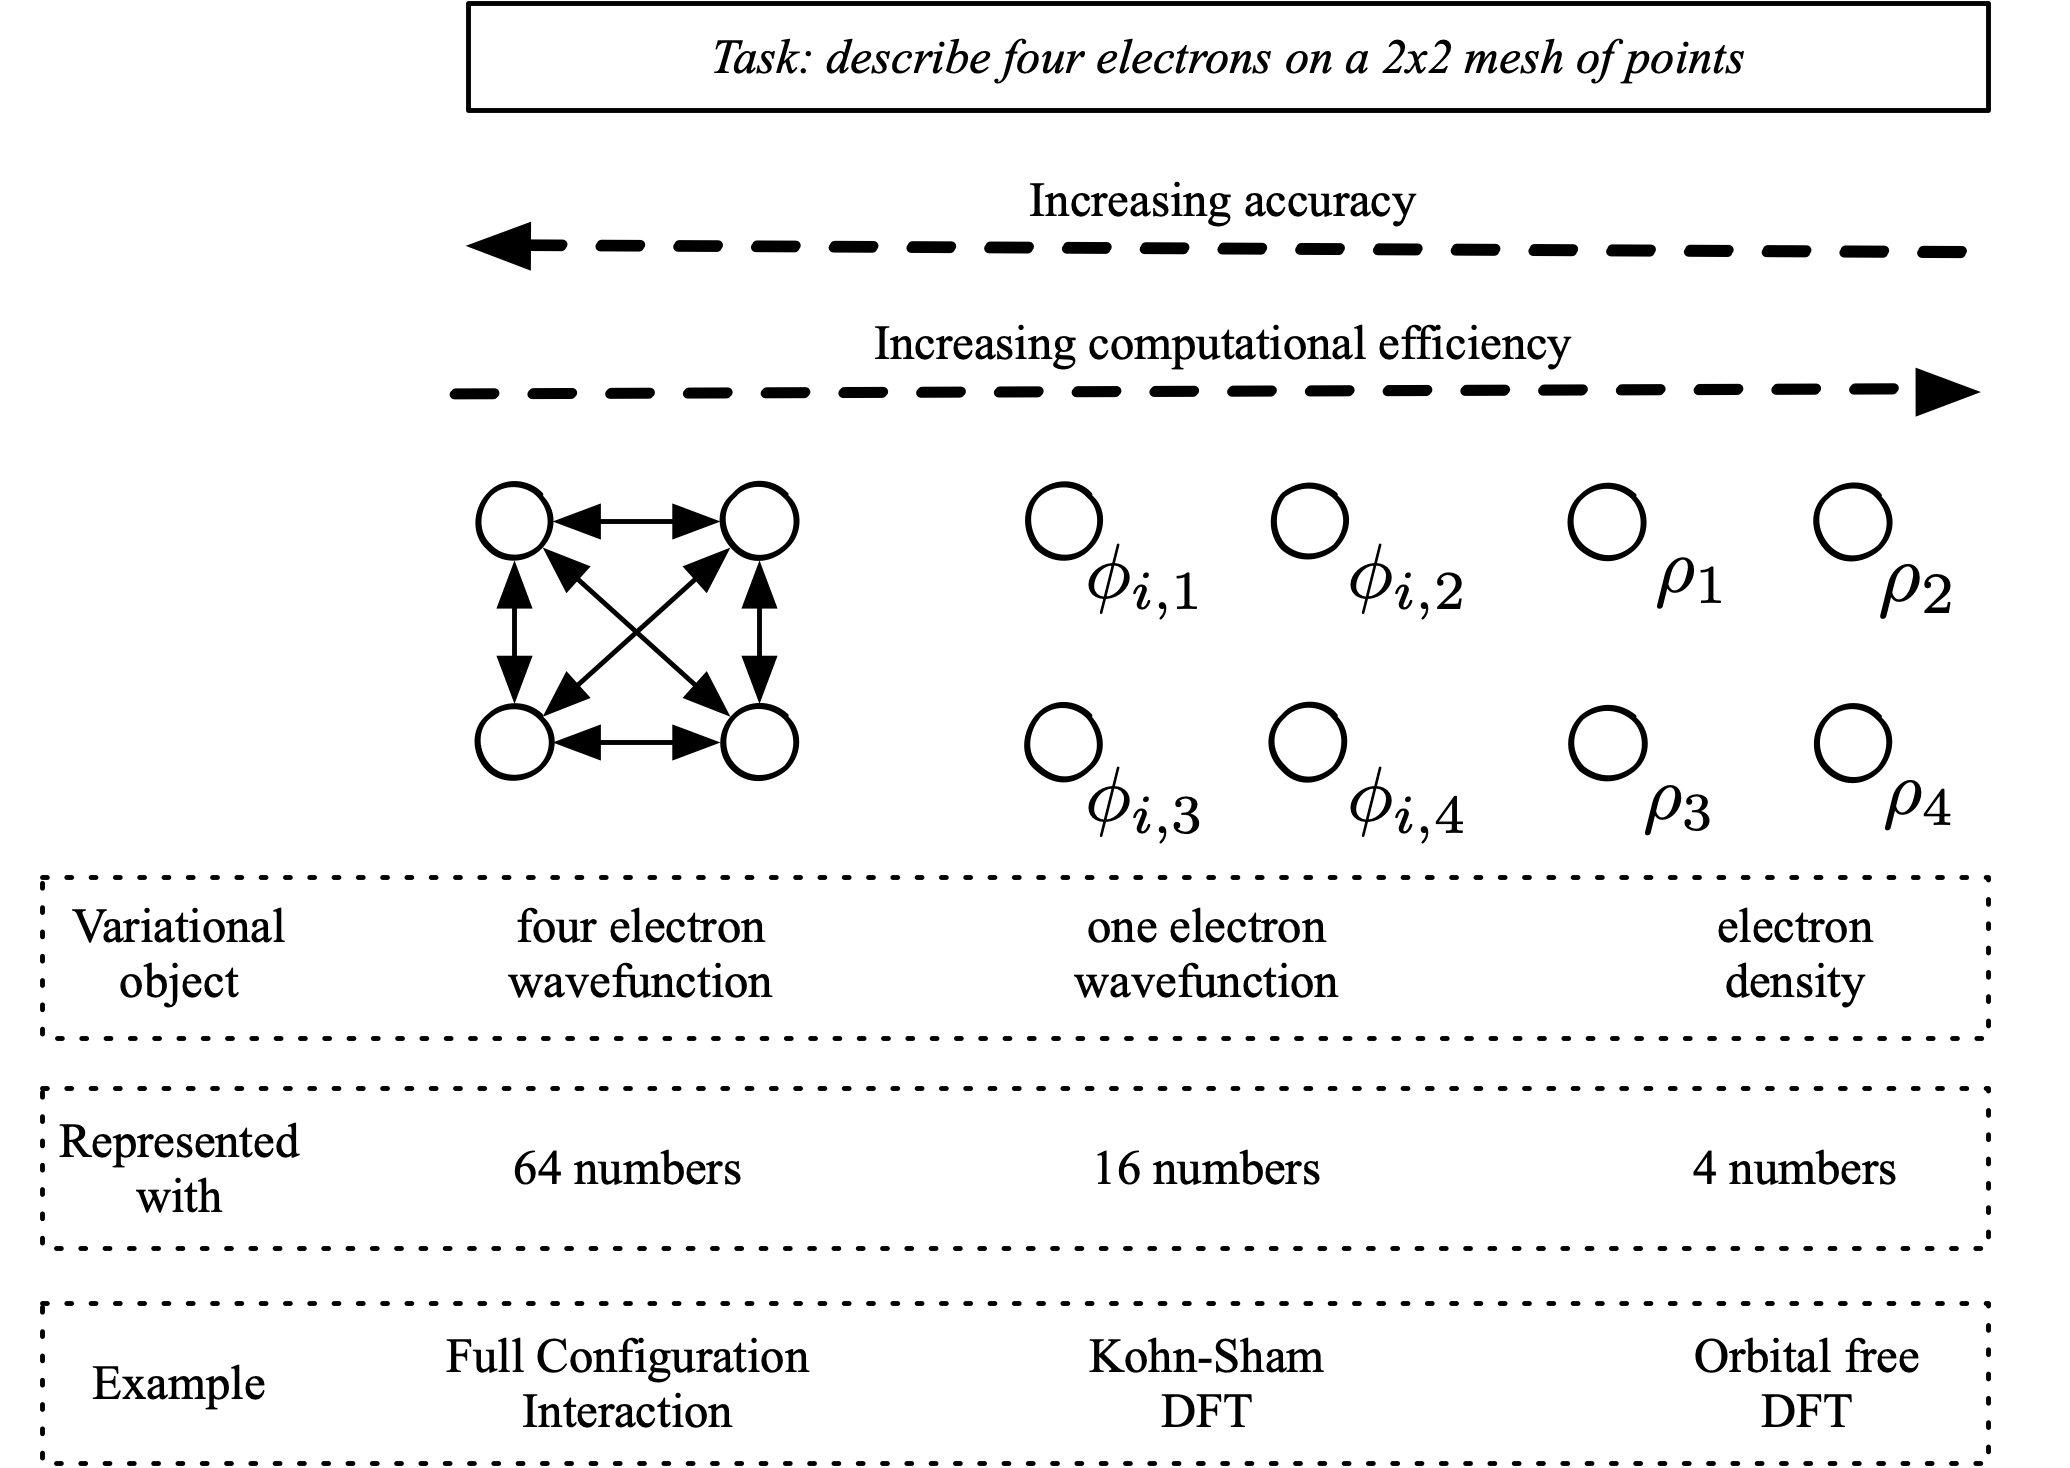
\includegraphics[resolution=450]{figures/ch3/dimensions.png}
  \caption[Dimensionality of variational objects]{To solve the Schr\"{o}dinger equation we can use a variational object with lower dimensionality and higher computational efficiency, although this will come at the cost of accuracy. This schematic is based on a discussion in Walter Kohn's Nobel Prize lecture.\autocite{Kohn1999}}
  \label{decouple}
\end{figure}
% Is this right? I don't understand how the two electron wavefunction scales (4^2) - it's discussed in the 14 easy lessons.


\subsubsection{The Kohn-Sham theorem} 

The Kohn-Sham theorem shows the for any interacting system with ground state density $\rho(\textrm{r})$ there exists a non-interacting system with the same ground-state $\rho(\textrm{r})$. To find the ground state energy of the real interacting system, the occupation numbers of \textit{fictitous}, non-interacting one-electron orbitals can be optimised. For a non-interacting system we know how to calculate $T\left[\rho\right]$ and this provides a good approximation to the true kinetic energy, so the Kohn-Sham theorem provide a more practical way to apply DFT. However, the exchange-correlation density functional $E_{\textrm{xc}}\left[\rho\right]$ is still not known. Only approximations to this functional can be made, leading to approximations for the electronic density, total energy and other system properties.


\subsection{DFT in practice}

\subsubsection{Exchange-correlation functionals}
To use Kohn-Sham DFT we must approximate the exchange-correlation functional, and there is a growing list of functionals with varying levels of complexity. A useful way of categorising these functionals, "Jacob's Ladder", has been proposed by John Perdew (Figure \ref{}). As a general rule, more accurate functionals are constructured by adding more parameters and variables.

\begin{figure}[h]
\centering
  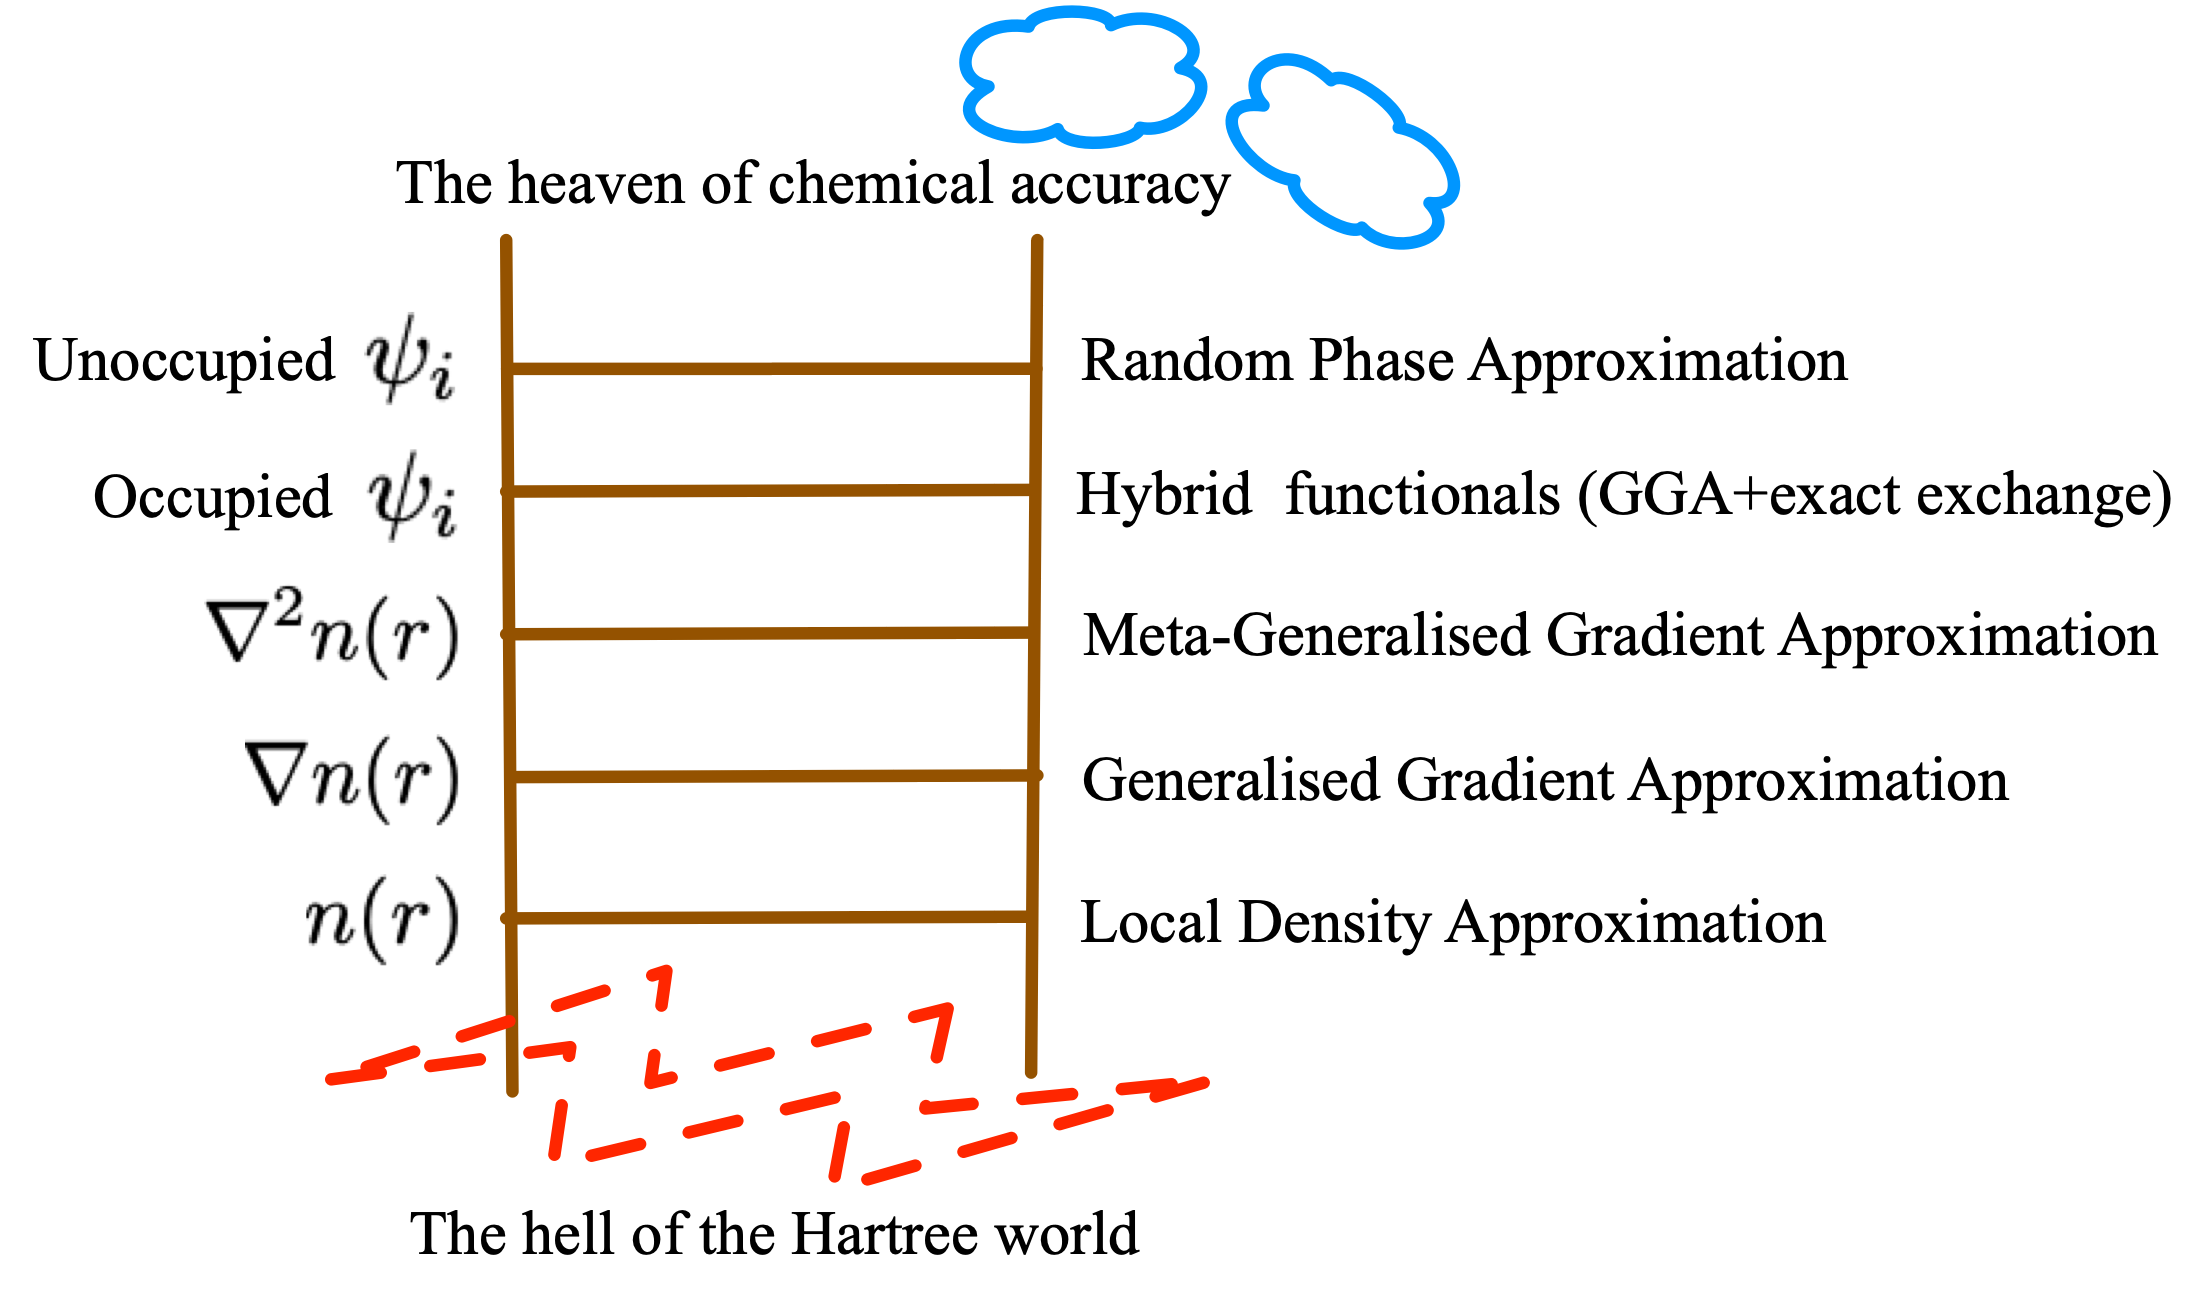
\includegraphics[resolution=450]{figures/ch3/jladder.png}
  \caption[Jacob's ladder of exchange-correlation functionals]{Jacob's ladder of exchange correlation functionals. On the right hand side are the various categories of exchange-correlation functionals and on the left hand side are the additional input variables included at each level of theory. As we move up the ladder the chemical accuracy increases, alongside computational expense.}
  \label{decouple}
\end{figure}

\textit{Local Density Approximation} \\
At the lowest rung of the ladder is the local density approximation. In this approximation, only one variable is used to calculate the exchange correlation energy. This is the charge density for an infinitesimal 3-dimensional volume element. The exchange energy is calculated exactly
$$
E_{\textrm{LDA,x}}\left[n\right] = −\frac{3}{4}\left(\frac{3}{\pi}\right)^{\frac{1}{3}}n^{\frac{4}{3}}\left(\textbf{r}\right)d\textbf{r},
$$
and the correlation energy is calculated numerically by fitting to many-body quantum monte carlo studies for an inhomogeneous electron gas.%Ceperley and Alder
Strictly, the LDA should only be used for slowly varying densities, however it has performed surprisingly well for predicting the properties of a variety of atoms, solids and molecules. This is due to a cancellation of errors: LDA underestimates the exchange energy and overestimates the correlation energy. However there is a tendency for LDA to overestimate the binding energy and underestimate lattice parameters. This is a particularly pronounced problem in weakly bonded systems. Common LDA functionals include VWN and PW92.

\textit{Generalised Gradient Approximation} \\
At the next level of theory, two variables are used to determine the exchange-correlation energy: charge density and the density gradient. GGAs are semi-local functions due to their dependence on the gradient. The parameters of GGA functionals can be derived from physical constraints (non-empirical, as in the widely used PBE functional), or obtained from fitting procedures (empirical, as in the case of B88). GGAs improve the over-binding of LDA, but tend to underestimate the band gap of the material.

\textit{Meta-GGA} \\
Meta-GGAs extend the GGA functional to include the non-interacting kinetic energy density as an input to the functional. This is the calculated from the laplacian of the occupied electron orbitals.
% could include equation here perhaps (make sure consisstent with earlier).
A common meta-GGA functional is TPSS.

\textit{Hybrid functionals} \\
On the fourth rung, hybrid functionals combine GGA functionals with a proportion of the exact HF exchange energy. The simplest hybrid functional takes the form
$$
E_{\textrm{hybrid,xc}}\left[n\right] = \alpha E_{\textrm{exact,x}} + \left(1-\alpha\right)E_{\textrm{GGA,xc}}
$$
In some studies, the proportion of exact exchange is tuned to reproduce the property of interest correctly. For example, $\alpha=0.25$ is commonly used to correctly reproduce the band gap of the hybrid halide perovskite MAPI.% check the alpha is right
In DFT each electron interacts with itself as the potential derives from the total charge density of the system. This error is particularly pronounced for localised states, for example after the trapping of an electron or hole. By including a proportion of exact HF exchange hybrid functionals correct the self-interaction error and improve the accuracy of predictions.
% good stuff here incl. schematic: https://www.ncbi.nlm.nih.gov/pmc/articles/PMC4892865/#S3title
% - Linked to Koopman’s linearity:E(N) – E(N-1) = En
% See Janak 1978. 

\textit{Random Phase Approximation} \\
Closest to heaven is the Random Phase Approximation, which uses all of the Kohn-Sham orbitals (occupied and unoccupied) as input. Previous approaches fail when there are significant long range effects, as they have no information about the electron density far from an electron. The RPA is able to correctly predict long-range interactions between non-overlapping electron orbitals, for example van der Waals interactions.

% can I find plot of total energy as function of seperation using different approaches??
%As DFT is exact except for the approximation to the exchange-correlation functional, any shortcoming to a DFT prediction can be attributed to the XC-functional. It should be noted though that DFT 
% DFT was not designed to calculate band gaps.
% - However, since 2000 functionals have been better at giving total energy but they don’t give accurate density: straying away from ab-initio into a fitting exercise: DFT is straying from the path towards an exact functional

\subsubsection{Exploiting symmetry}

The material studied in this thesis, \ce{CH3NH3PbI3}, is a crystalline solid. Although we want to understand the properties of a finite piece of material, we use the standard approach which is to model the finite crystal as an infinite crystal. This is acceptable if the crystal piece is large enough so that it's properties do not depend on size. We introduce Born-von Karman (periodic) boundary conditions so that the infinite crystal is built from a repeating array of unit cells. For a unit cell of length $L$, any physically significant function $\psi$ of the crystal must have the same value at the origin and $L$, or in 3D:

\begin{equation}
\psi([0 0 0]) = \psi([L 0 0]) =  \psi([ 0 L 0]) = \psi([0 0 L])
\end{equation}

where the square bracket denotes a vector on the basis of the three unit cell vectors (Figure \ref{translational}. Note that there are an infinite number of unit cells of different shapes and sizes that can be used to build an infinite crystal.

It is often the case that translational symmetry is broken in the real material, for example when there are point defects (as in Results chapter \ref{}). Furthermore, lattice vibrations have a periodicity larger than the unit cell (Results chapter \ref{}). To model this phenomena a supercell is built from multiple unit cells and this is used as the basic repeating unit (Figure \ref{translational}).

\begin{figure}[h]
\centering
  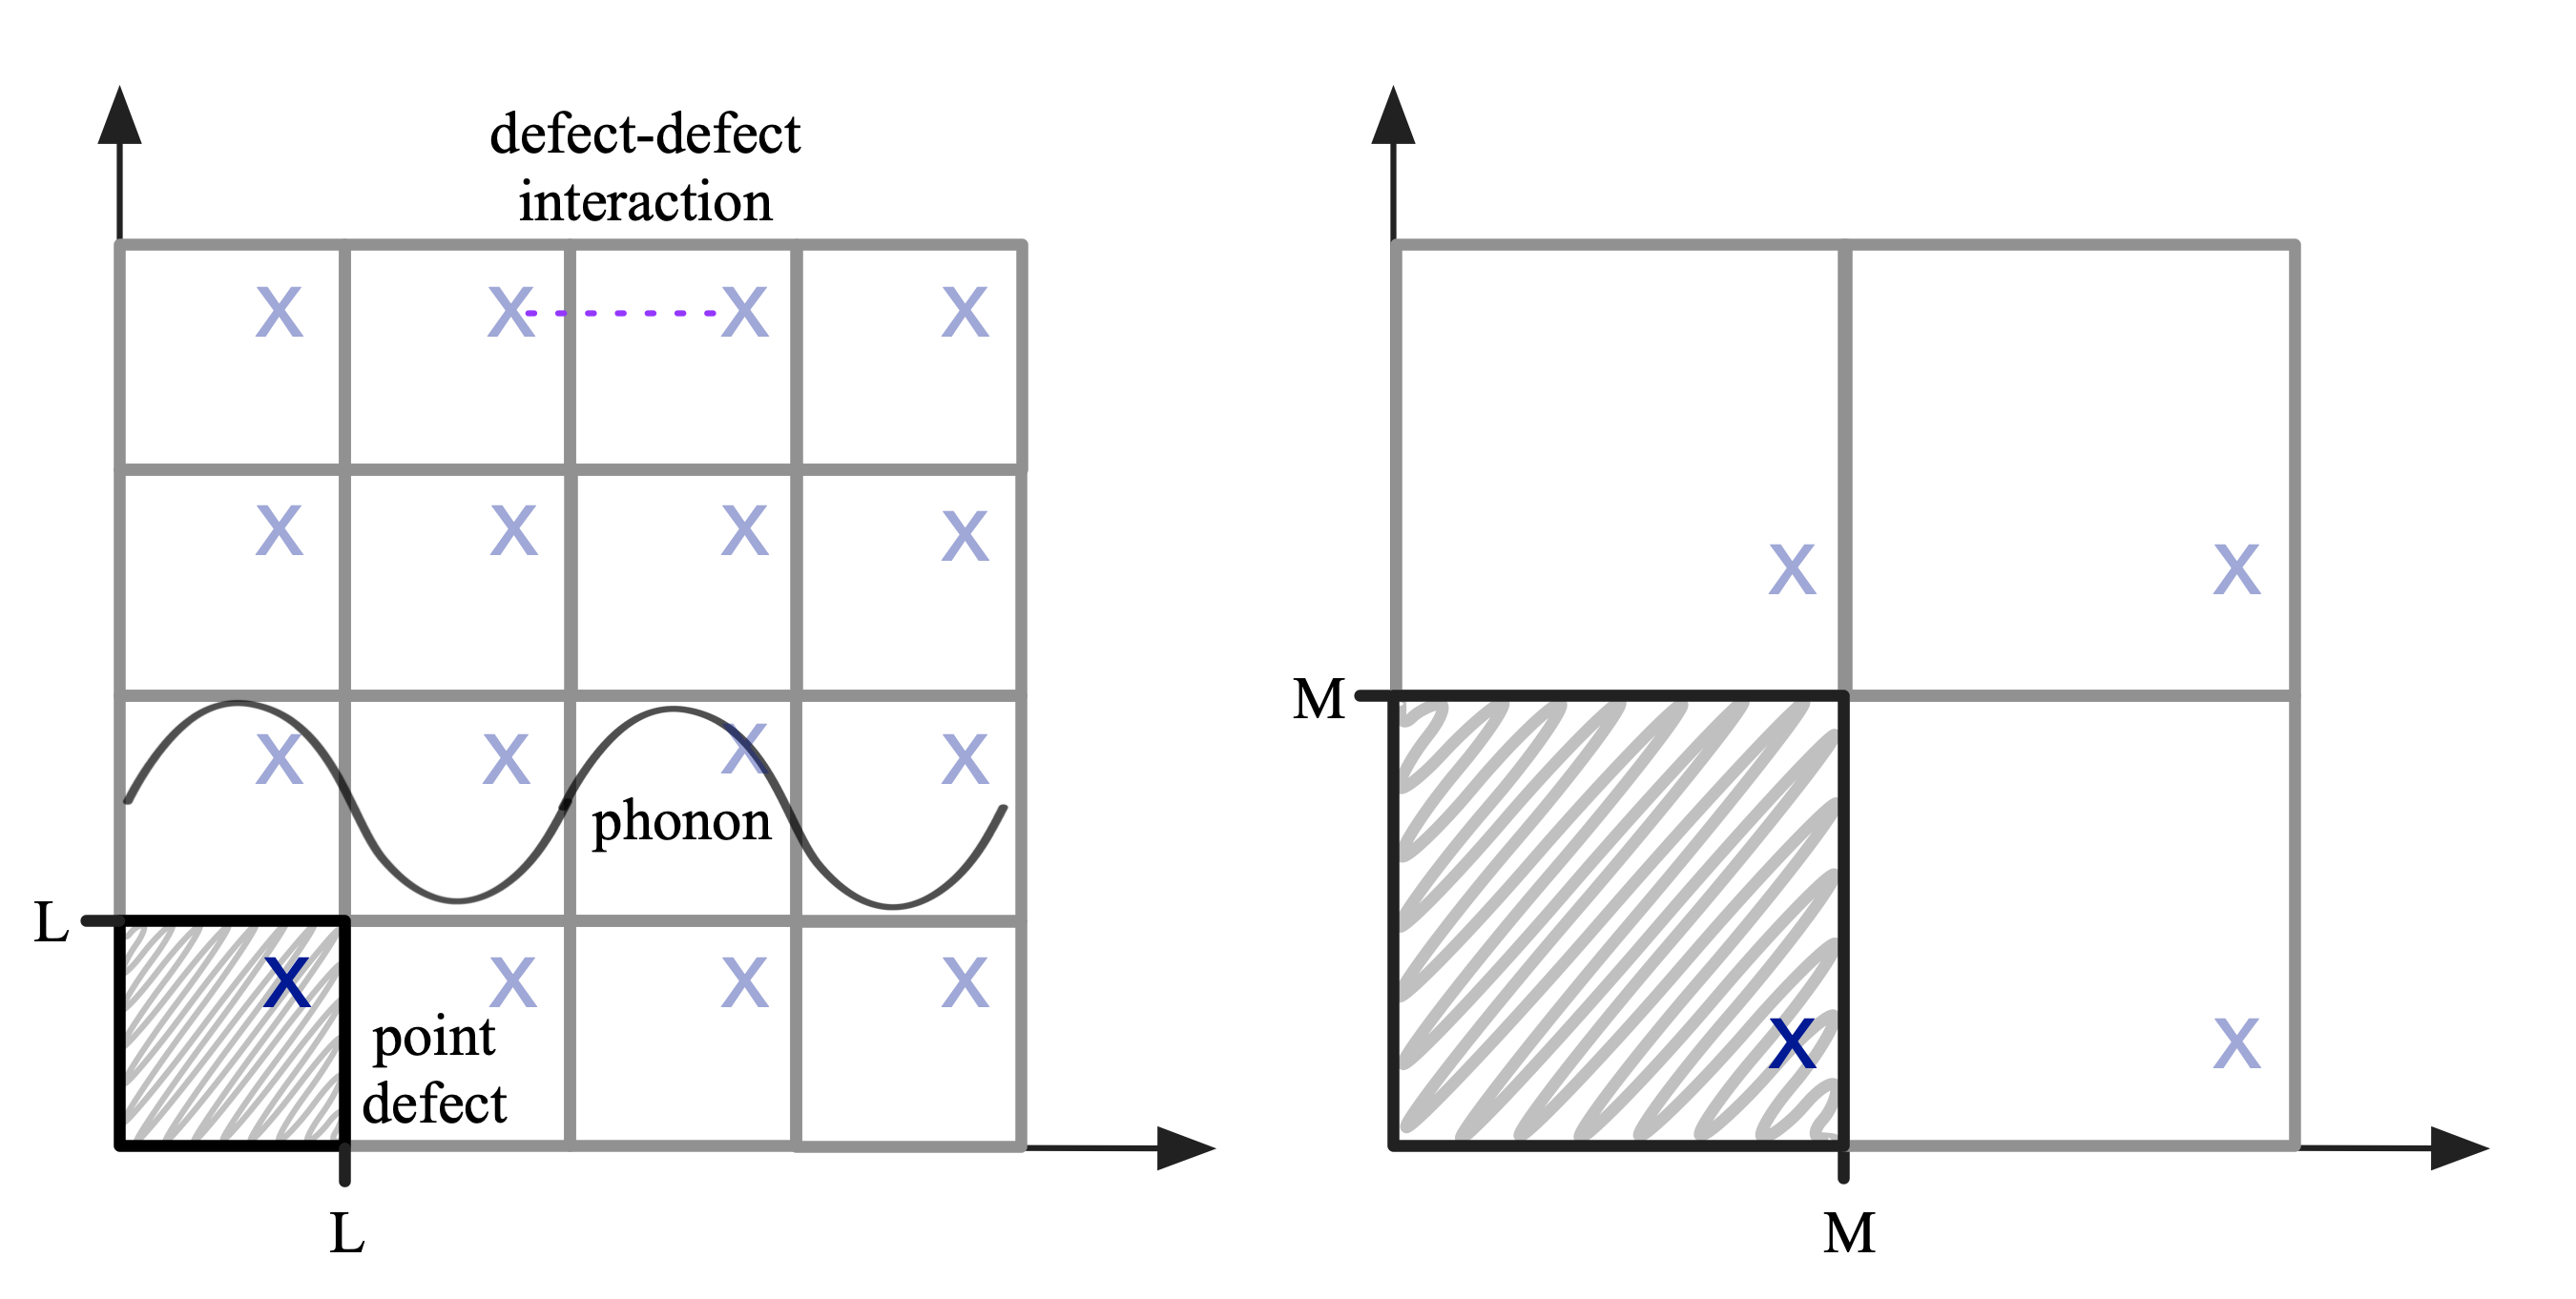
\includegraphics[resolution=450]{figures/ch3/supercell.png}
  \caption[Translational symmetry and supercell construction]{An infinite crystal is built from a repeating unit cell of length $L$ (LHS). Point defects (marked with an `x') break translational symmetey in real crystals and care must be taken when modelling these as neighbouring defects can interact with each other in an unphysical way. In addition, vibrational modes can have wavelengths $>L$ (sine wave). A supercell of length $M=2L$ can be built to better model these effects (RHS). } 
  \label{translational}
\end{figure}
% copy and paste phonon mode across to supercell picture?

When the Schrodinger equation is solved for a H atom the solution gives wavefunctions corresponding to the 1s, 2s, 2p, etc orbitals found in chemistry. For periodic systems, wavefunctions are formed by Bl\"{o}ch functions:\autocite{Hoffman1987}

\begin{equation} 
\psi_{k} = u_ke^{i\textbf{k}\cdot\textbf{r}}
\label{bloch}
\end{equation}   %could do a sketch of the two parts and the resulting part, and the periodic potential

where the Bl\"{o}ch function is formed from the product of a function $u_k$ with the same periodicity as the crystal lattice, and a plane wave $e^{i\textbf{k}\cdot\textbf{r}}$. $k$ is a crystal wave vector which forms a space known as reciprocal space; to understand the physical significance of $k$ we consider an infinite 1D chain of hydrogen atoms separated at distance $L$ (Figure \ref{bands}). The electron states can be described a linear combination of H 1s orbitals $u_n$ centred at each lattice point :

\begin{equation}
\psi_k = \sum_nu_ne^{inkL}
\end{equation}

$k=0$ corresponds to the low energy most bonding state, and $k=\frac{\pi}{L}$ corresponds to the high energy anti-bonding state
\begin{align}
\psi_0 &= \sum_nu_ne^0 = u_1 +u_2 +u_3 +u_4 \dots \\
\psi_{\frac{\pi}{L}} &= \sum_nu_ne^{i\pi n} = u_1 -u_2+u_3-u_4 \dots
\end{align}
Between these two extremes there is a continuum of states forming an electronic band (Figure \ref{bands}). 

Substituting Equation \ref{bloch} into Equation \ref{singleparticle} gives

\begin{equation} \label{energyequation}
\left[\frac{1}{2m}\left(\frac{\hbar}{i}\nabla+\hbark\right)^2+V(\textbf{r})\right]u_k = E(k)u_k
\end{equation}

For any $k$ we can solve Equation \ref{energyequation} with periodic boundary conditions to find the bandstructure $E(k)$. The bandstructure is often modelled as being parabolic around the maxima and minima, and the curvature determines the carrier effective mass which is explored in Chapter \ref{ch:4-effmass}. There are an infinite number of eigenvalues so the energy is labelled $E_n(k)$ where n labels the particular eigenvalue (band). As a result of crystal symmetry, $E_n(k)$ is periodic and only $k$-vectors within a region of space known as the Brillouin Zone ($|k|<\frac{\pi}{a}$) need to be considered. %I should cite the transport booked used, and include modelling as parabola to link to effective mass.
%talk about high symmetry points and the naming conventions (greek in zone and latin a boundaries) - choose route through use aflowlib

\begin{figure}[h]
\centering
  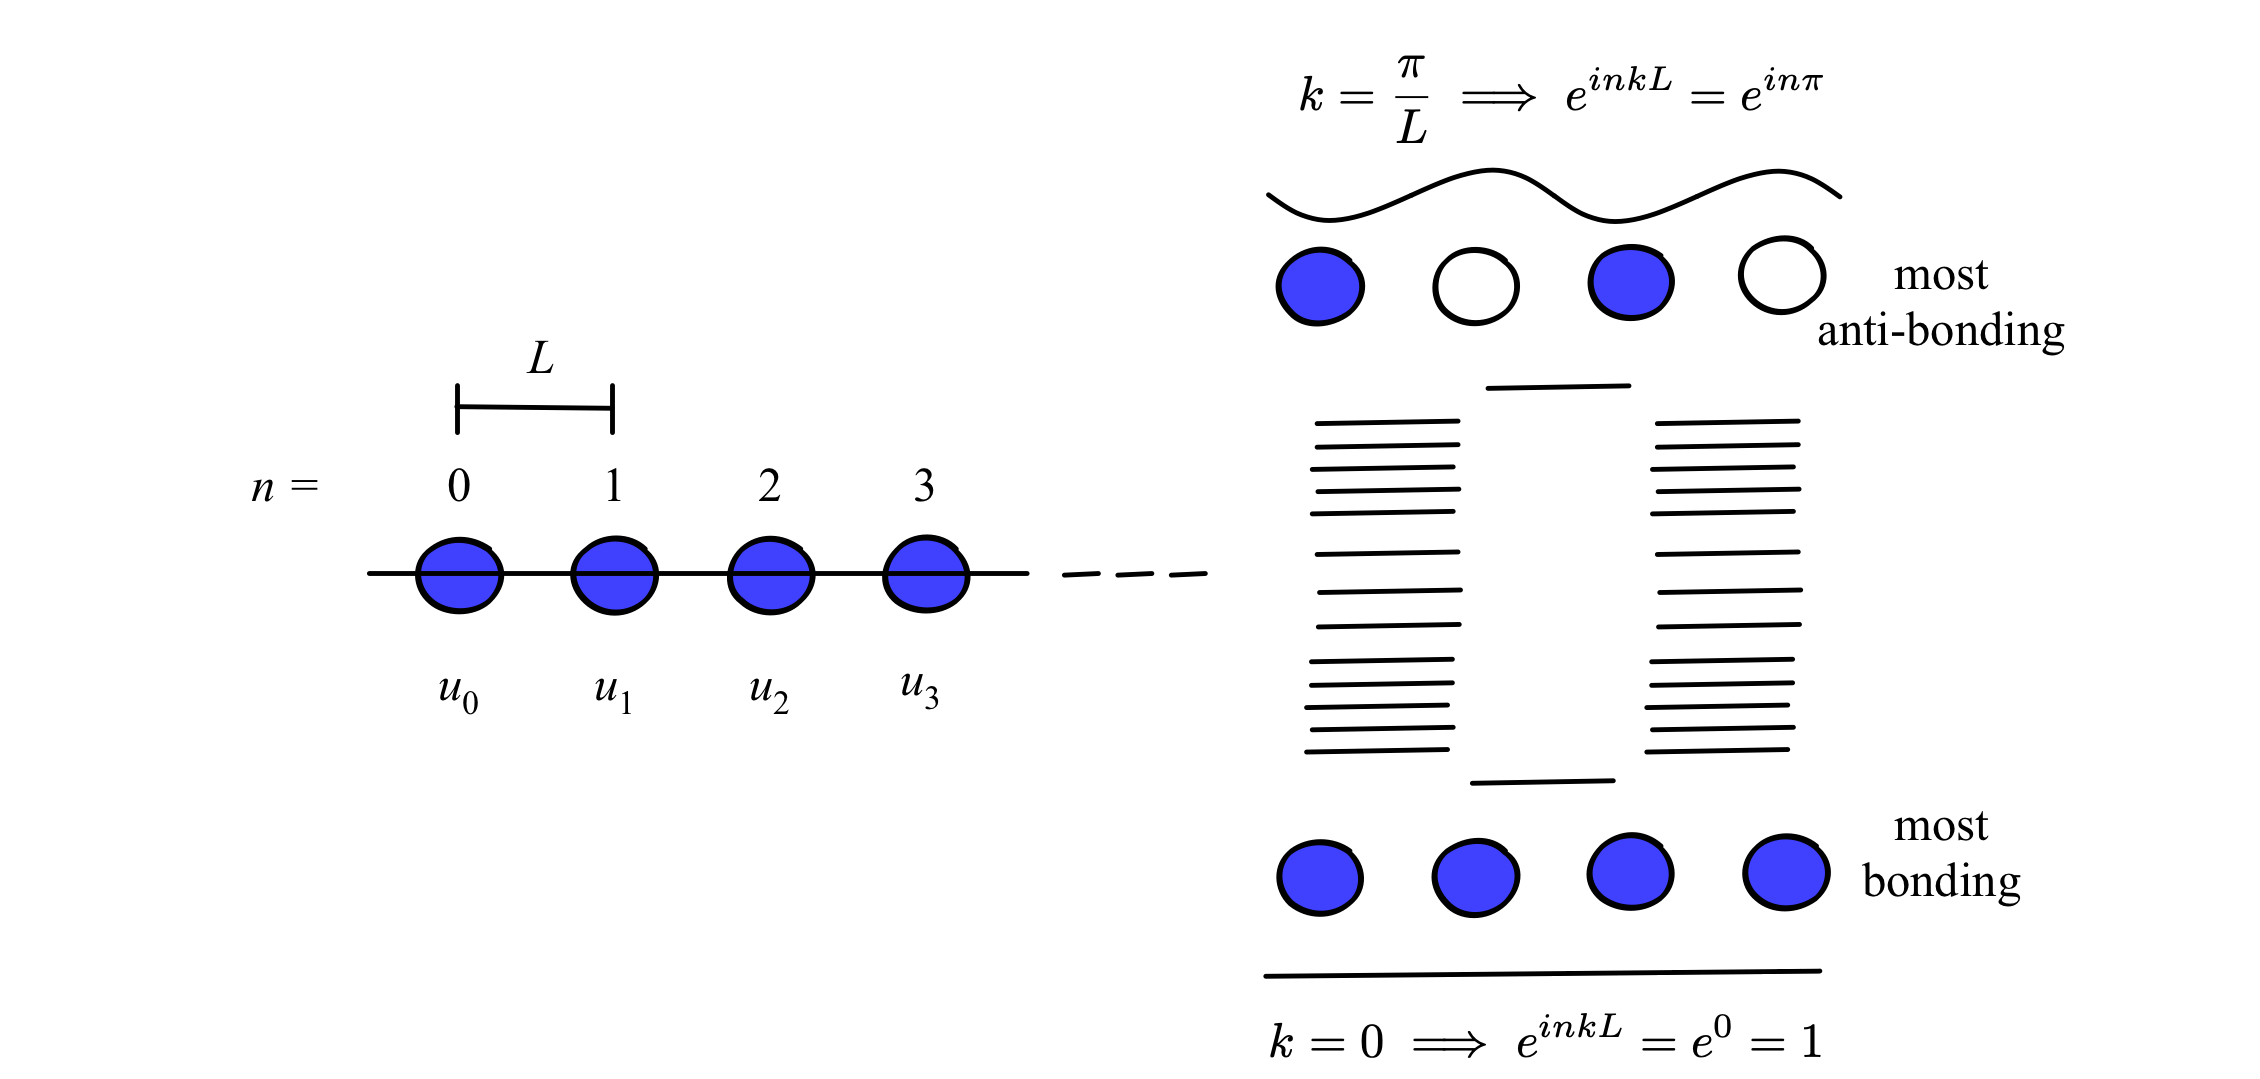
\includegraphics[width=1.0\columnwidth]{figures/ch3/bands.png}
  \caption[]{} 
  \label{bands}
\end{figure}

\subsubsection{Basis Sets}   %valence bands and conductions bands?

In the previous example the lattice periodic part of a bloch function took the form of a H 1s orbital. For more complex systems, $u_k$ can itself be expanded into a plane wave basis set whose wave vectors $G$ are reciprocal lattice vectors

\begin{equation}
u_k = \sum_Gc_{\textbf{k},\textbf{G}}e^{i\textbf{G}\cdot\textbf{r}}.
\end{equation}

The complete expanded Kohn-Sham wavefunction can be expressed as

\begin{equation} \label{KSeigenstates}
\psi_k = \sum_Gc_{\textbf{k},\textbf{G}}e^{i(\textbf{k+G})\cdot\textbf{r}}
\end{equation}

A plane wave basis set is often used for extended systems as they are inherently peroidic. The software used for the DFT calculations in this thesis, \ce{VASP}\autocite{}, uses a plane wave basis set. For DFT calculations applied to localised systems, such as molecules or nanoparticles, localised basis sets such as gaussian orbitals can be used. This is implements in software such as \autcite{}.

Sudden changes in electron density are hard to capture using a plane wave basis set (to take the extreme example, the fourier decomposition of a simple top hat in real space needs requires an infinite summation in reciprocal space). This can be problematic when describing the region around the nucleus where there are strong oscillations in the wavefunctions. However these oscillations are associated with the core electrons which are less important in chemical bonding, and so pseudopotentials - an effective potential without oscillations - can be used. It has been established that for certain systems pseudopotentials are as precise as all-electron calculations.\autocite{Lejaeghere2016a}
%http://helper.ipam.ucla.edu/publications/maws3/maws3_6085.pdf
%http://davidbowler.github.io/AtomisticSimulations//blog/dft-reliability#R3

\subsubsection{Optimising the atomic and electronic structure}

In this section the process of optimising the atomic and electronic structure of a system towards the ground-state (minimum energy) configuration is outlined. 

In Section \ref{DFTtheory} (Figure \ref{decouple}) we saw that the potential $v_\textrm{ee}$ is dependant on electron density $\rho$, which is itself dependant on $v_\textrm{ee
}$. Therefore an iterative approach, the Self Consistent Field (SCF) method, is used to calculate the ground-state electronic structure (Figure \ref{SCF}, dashed section). The initial guess for the density $n(r)$ is given by a superimposition of the atomic charge densities. This is used to calculate the potential and solve the KS equations, which gives a new $n(r)$. This process continues until the convergence criteria is met (most often within an energy tolerance). Various optimisation routines are provided in DFT codes for finding the ground state configuration, including the conjugate gradient scheme, Davidson Scheme and RMM-DIIS.

DFT is also used to find the ground state atomic structure. Structures from X-ray Diffraction Data are used as a starting guess, so that finding the energetic minimum becomes a local optimisation problem. Ions in the systems are displaced (either the internal coordinates of the unit cell or the unit cell parameters themselves are adjusted) and the electronic structure for that geometry is solved self-consistently. This repeats until the forces on each atom are zero (within a given tolerance, Figure \ref{SCF}). 
%optimisation routines.
% Talk about the PES here

\begin{figure}[h]
\centering
  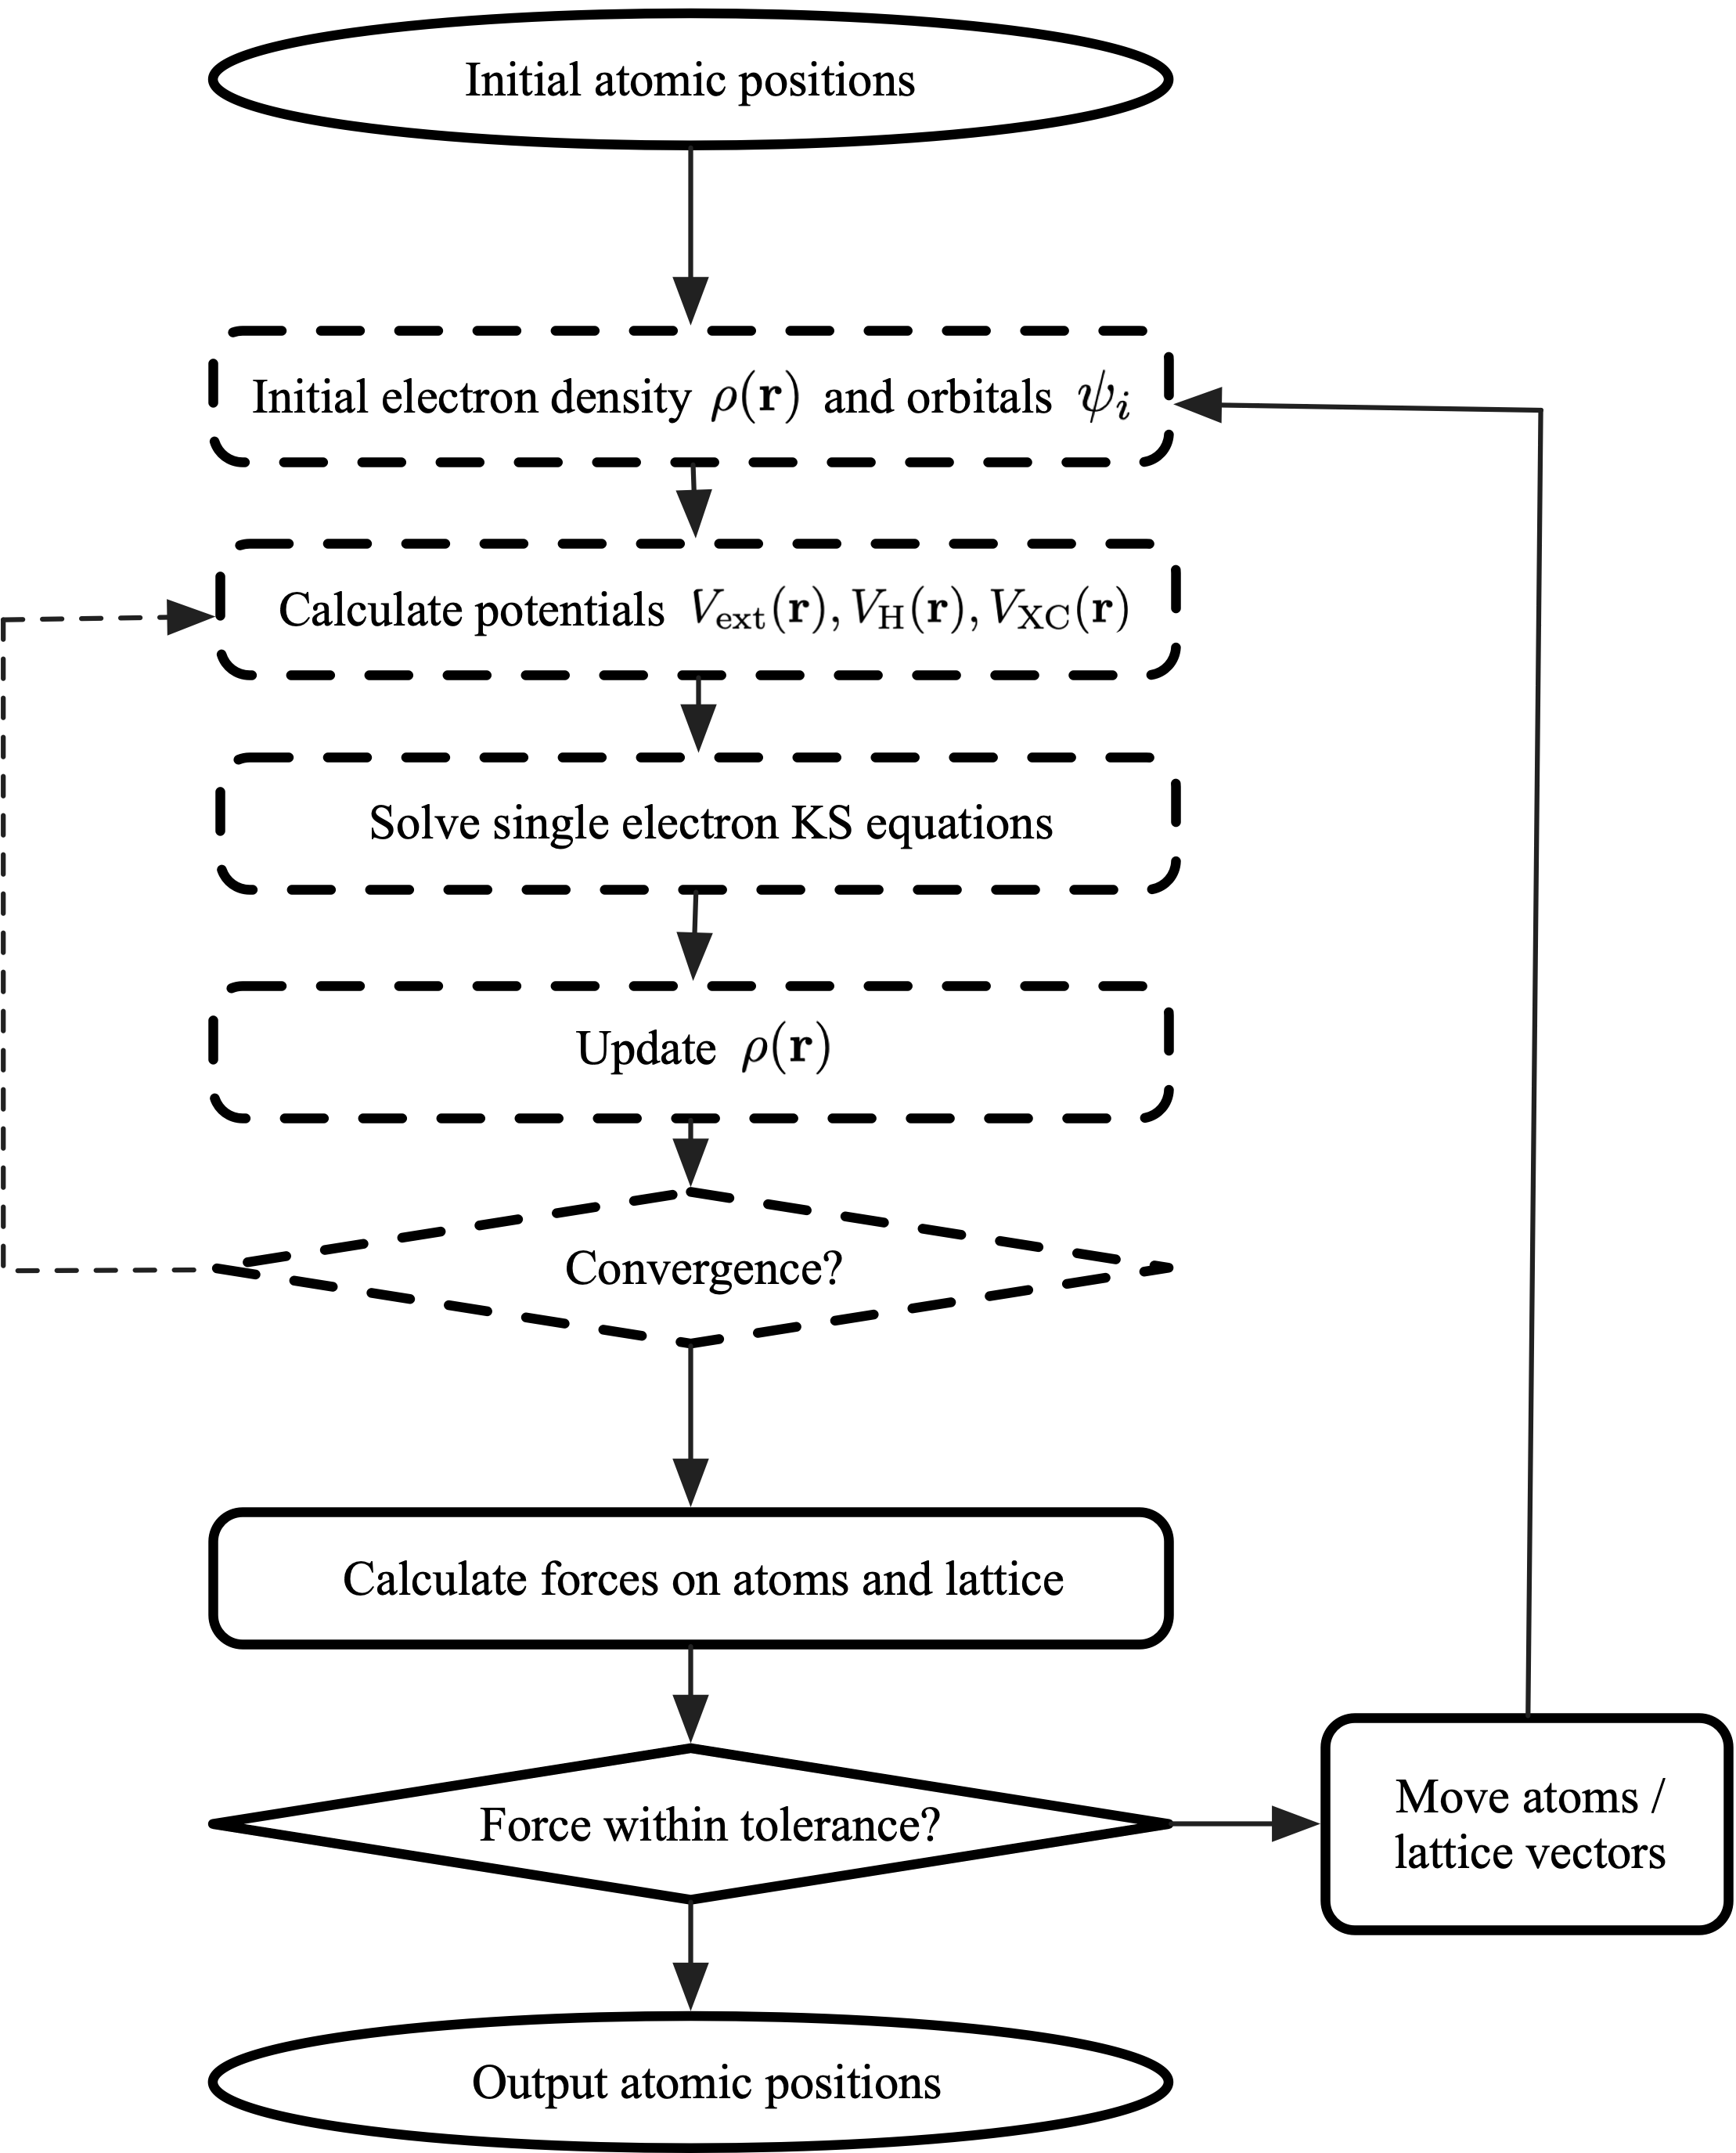
\includegraphics[resolution=450]{figures/ch3/scf.png}
  \caption[Nested iterative method for geometry optimisation]{Nested iterative method for geometry optimisation. The electronic structure relaxation (dashed lines) is nested within the atomic structure relaxation (solid lines).} 
  \label{SCF}
\end{figure}
%% the potentials aren't correct need to fix this and addd potentials explicitly to the DFT part of the theory
\subsubsection{The limits of DFT}

\textit{Thoeretical limitations}

In Section \ref{DFTtheory} we outlined the approximations inherent to DFT calculations: the Born-Oppenheimer approximation and the unknown exchange-correlation functional. Higher levels of theory, which incorporate the effects of spin and relativity (e.g. spin-oribt coupling) are included in many DFT implementations. However DFT is still restricted to ground-state properties and higher levels of theory (GW or TDDFT) are required to describe optical excitations, for example. Another inherent limitation is that the KS eigenvalues are artificial; only the ground state electron density and derived properties are correct. In practice, the KS eigenvalues are used to calculate the band gap, although quantitative band gaps often require the use of hybrid functionals which are tuned to give the correct band gap.

\textit{Numerical limitations}

There is also a different set of approximations that relate to  numerical convergence rather than the underlying theory.

First, we have seen that the Kohn-sham wavefunctions are expanded in a basis set. In principle an infinite set may be needed to describe the Kohn-Sham wavefunction; in practice the basis set must be truncated. The kinetic energy operator is given by $-\frac{\hbar \Nabla^2}{2m}$. When this is applied to the plane wave Kohn-Sham eigenstates as given in Equation \ref{KSeigenstates}, we find that the kinetic energy is proportional to $|k+G|^2$; faster oscillations correspond to higher energy. A cutoff energy $\textrm{E}_\textrm{cut}$ is defined so that
\begin{equation}
\frac{1}{2}|k+G|^2 < \textrm{E}_\textrm{cut}.
\end{equation}
This cutoff energy must be tested to ensure that the property of interest, most often energy, is converged to within a certain range.

Second, to calculate many properties of interest we need to integrate over the Brillouin Zone. To calculate the total energy of an insulator for example, we use
\begin{equation} \label{energyintegral}
    E = \frac{\Omega}{(2\pi)^3}\sum_\textrm{occ.}\int_\textrm{BZ}E(\textbf{k})d^3k
\end{equation}
where $\Omega$ is the volume of the Brillouin zone and there is a sum over all occupied bands. 
In practice we do not know the continuous form for $E(\textbf{k})$ and so we evaluate Equation \ref{energyintegral} numerically as a weighted sum over special points in reciprocal space which form a $k$-point mesh. This is often an equally spaced mesh centred on the $\Gamma$-point ($k=(0,0,0)$) in reciprocal space. For any given system, the $k$-point density scales inversely with cell size; if the unit cell in Figure \ref{translational} requires a $6\times6$ $k$-point grid, the $2\times2$ supercell requires a $3\times3$ $k$-point grid. As with plane waves, there is a balance between accuracy (the higher the number of $k$-points, the higher the accuracy) and computational expense. An example convergence study is given in Figure \ref{kpointconvergence} where a $5\times5\times5$ $k$-point grid is required to converge pressure to within \SI{1}{\kilo\bar} and energy to within \SI{0.1}{\electronvolt} in \ce{CsSnI3}.

\begin{figure}[h]
\centering
  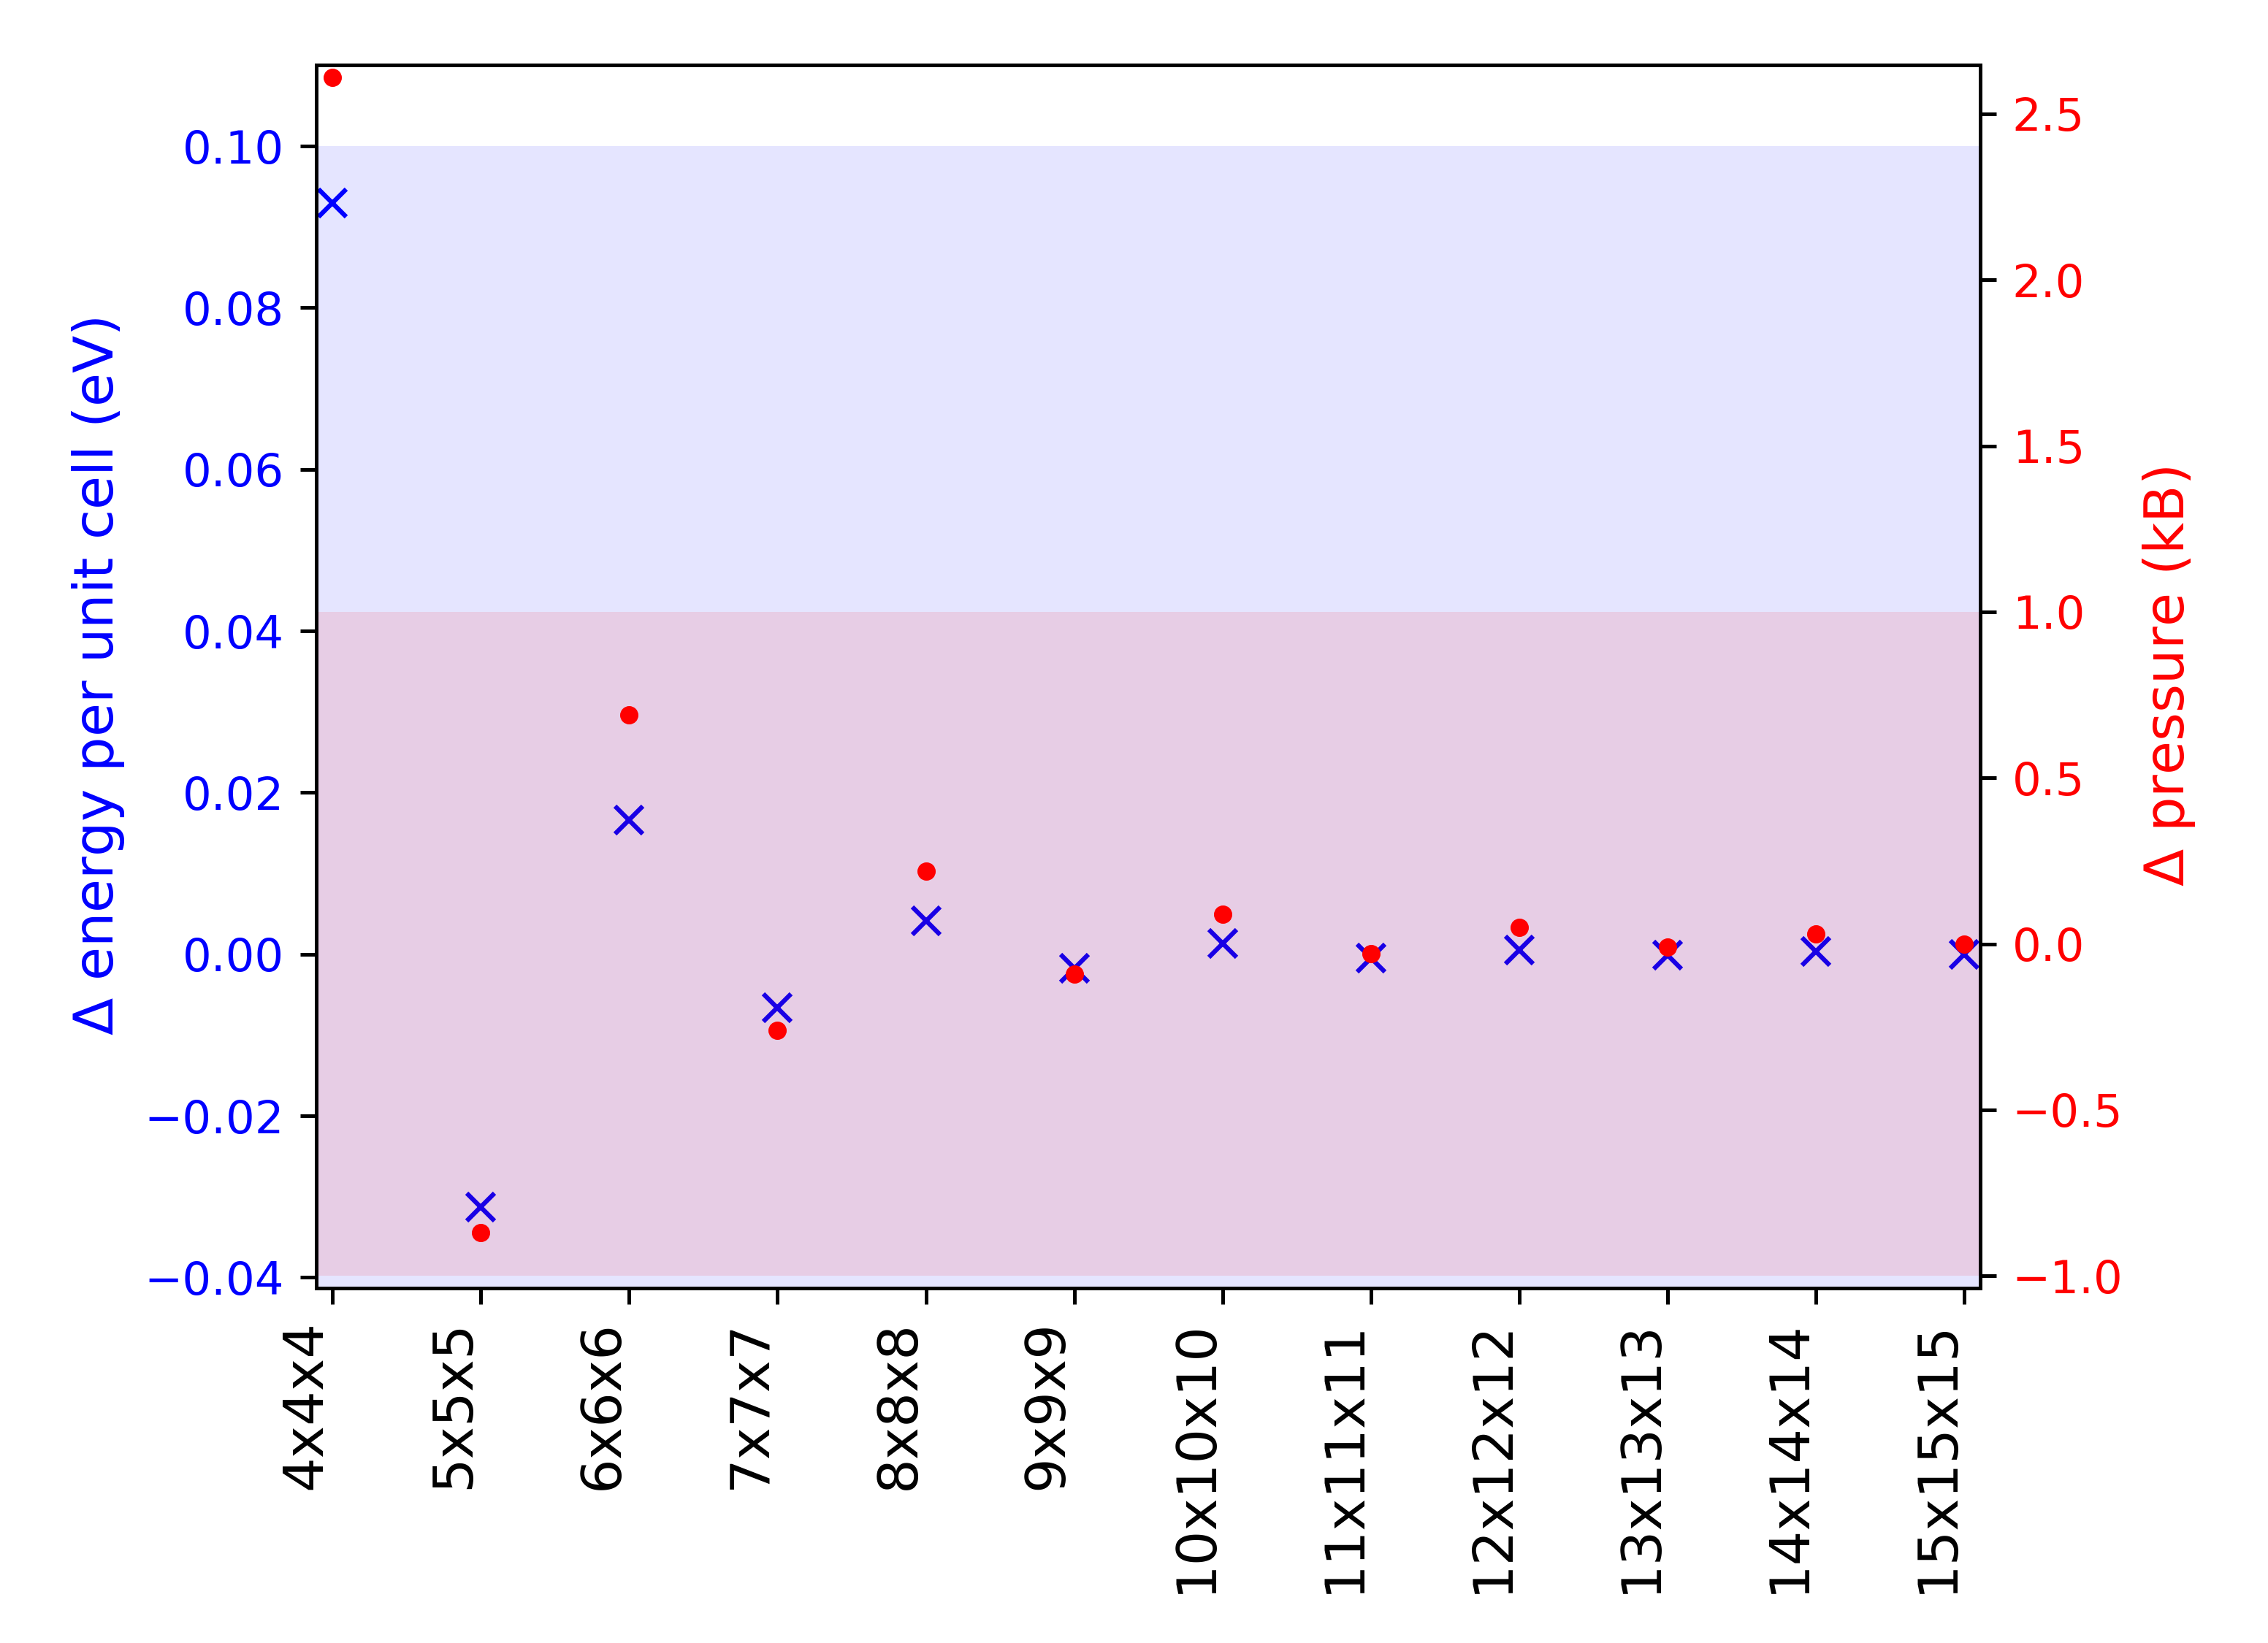
\includegraphics[resolution=450]{figures/ch3/kpointconvergence.png}
  \caption[$k$-point convergence of \ce{CsSnI3}]{$k$-point convergence of \ce{CsSnI3}. The $k$-point grid size is on the $x$-axis. Pressure is denoted with a red dot; the region which is within the \SI{1}{\kilo\bar} convergence criteria for this study is shaded red. Energy is denoted with a blue cross; the region which is within the \SI{0.1}{\electronvolt} convergence criteria  is shaded in blue. Only odd grids sample the $\Gamma$-point and so there is an oscillation in energy and pressure as we move between odd and even grids.}
  \label{kpointconvergence}
\end{figure}

% - K-point grids and the commensurate grids for supercells.
% - Doubles k-points reuired as k and –k now no longer equivalent (SoC?)
%All convergence tests must be done for the property of interest. Cancellation of errors can mean that energy differences converge faster than ground state energies, as is reported in Chapter \ref{}.   % EP coupling calcas 
% - See: Designing meaningful density functional theory calculation in materials science - a primer Anne E Mattson et al. Model. Sim. Mater. Sci Eng. 13 R1-R31 (2005). : for information about convergence and getting meaningful results.

%\textit{Computational limitations}
% - history of computers section at science museum for HPC section
% - put the amount of computer time and carbon burnt here?
% - computational expense: limitations on size: See review of materials models which Alison Walker mentions. Mesoscopic bridges the atomistic with the drift diffusion models. Meso is often monte carlo, tranjectory tpe calculations. Cells are too big for atomistic (1 cm squared). Efficiecny depends upon J-V curves which can only be modelled at scale of fill device. The electrostatics is incredible important which linked ot build up of charges at SC nd OC. Grain boundaries and recombination at intercaes.





\clearpage

\section{Calculating the properties of defects in semiconductors}

The second law of thermodynamics states that "an isolated system tends towards an equilibrium macrostate with maximum entropy". A consequence of this is that all solids in equilibrium at finite temperature contain point defects, as the cost in lattice energy is balanced by the change in configrational entropy. 
Point defects are associated with a number of microscopic processes that can be beneficial or detrimental to material performance, including:
\begin{itemize}
    \item optical: colour centres, up/down conversion
    \item electrical: conductivity, carrier trapping, ionic hopping
    \item mechanical: material hardening
    \item thermal: conductivity, decomposition
\end{itemize}
The wide ranging impact of point defects accounts for the continuing research activity that began in 1926 when Yakov Frenkel introduced the concept of defects in a crystalline structure. Theoretical methods are particularly useful in this field as, although it is relatively straight forward to estimate the quantity of defects in a material, it is much more challenging to identify the type of defect.  
 
. In this section I first outline the different types of crystal defects, and then discuss the thermodynamics of (charged) defect formation. I end the section by outlining the supercell method for calculating defect properties. This method was used in Chapter \ref{ch:6-defects}, where I calculate electronic structure properties which lead to a description of the defects in \ce{Ch3NH3PbI3}.
% We are interested in calculating the electronic structure properties which lead to a description of the defects (trap density, binding energy, trap level, capture cross section).

% cite defects and defect processes in nonmetallic solids

% - History:
% - 1912 Born and Karman . PBC (first lattice dynamics paper)
% - 1925 Frenkel – formation of frenkel pair (first defects paper)
% - 1922 Jost – probability of forming defects. Tied into experimental work popular at the time, looking at how a material can be an ionic conductor when it is electrically insulating
% - 1938 Mott – the Mott-Littleton approach for calculating defects

\subsection{Classification of crystal defects}

The first way to classify defects is via their dimension. 0-dimensional are localised around isolated sites in the crystal and are known as point defects. 1-dimensional are lines along which the crystal pattern is broken and are called dislocations. 2-dimensional defects are surfaces along which distinct crystallites are joined and are called grain boundaries or interfaces. 3-dimensional defects are changes to the crystal pattern in finite volumes, this includes precipitates and voids. 

The remainder of this thesis concerns 0-dimensional point defects, which can be further split into extrinsic or intrinsic defects. Extrinsic point defects are impurity atoms, different from the host species. These defects may be added intentionally (for example, to increase electrical conductivity) or unintentionally (as a result of the fabrication method). Intrinsic point defects are associated with host species.

Point defects can also be classified as non-stochiometric or stochiometric. Non-stochiometric defects include interstitials (where an additional atom occupies a site that is unoccupied in the perfect lattice), vacancies (missing atoms) and anti-sites (where atom occupies a site that is occupied by another species in the perfect lattice). Interstitials can have a ``split'' structure, in which two atoms are split symmetrically around a single lattice site. Stochiometric defects include Frenkel pairs, Shottky pairs and V-centres. The stochiometric and non-stochiometric defects are illustrated in Figure \ref{classification}.

\begin{figure}[h]
\centering
  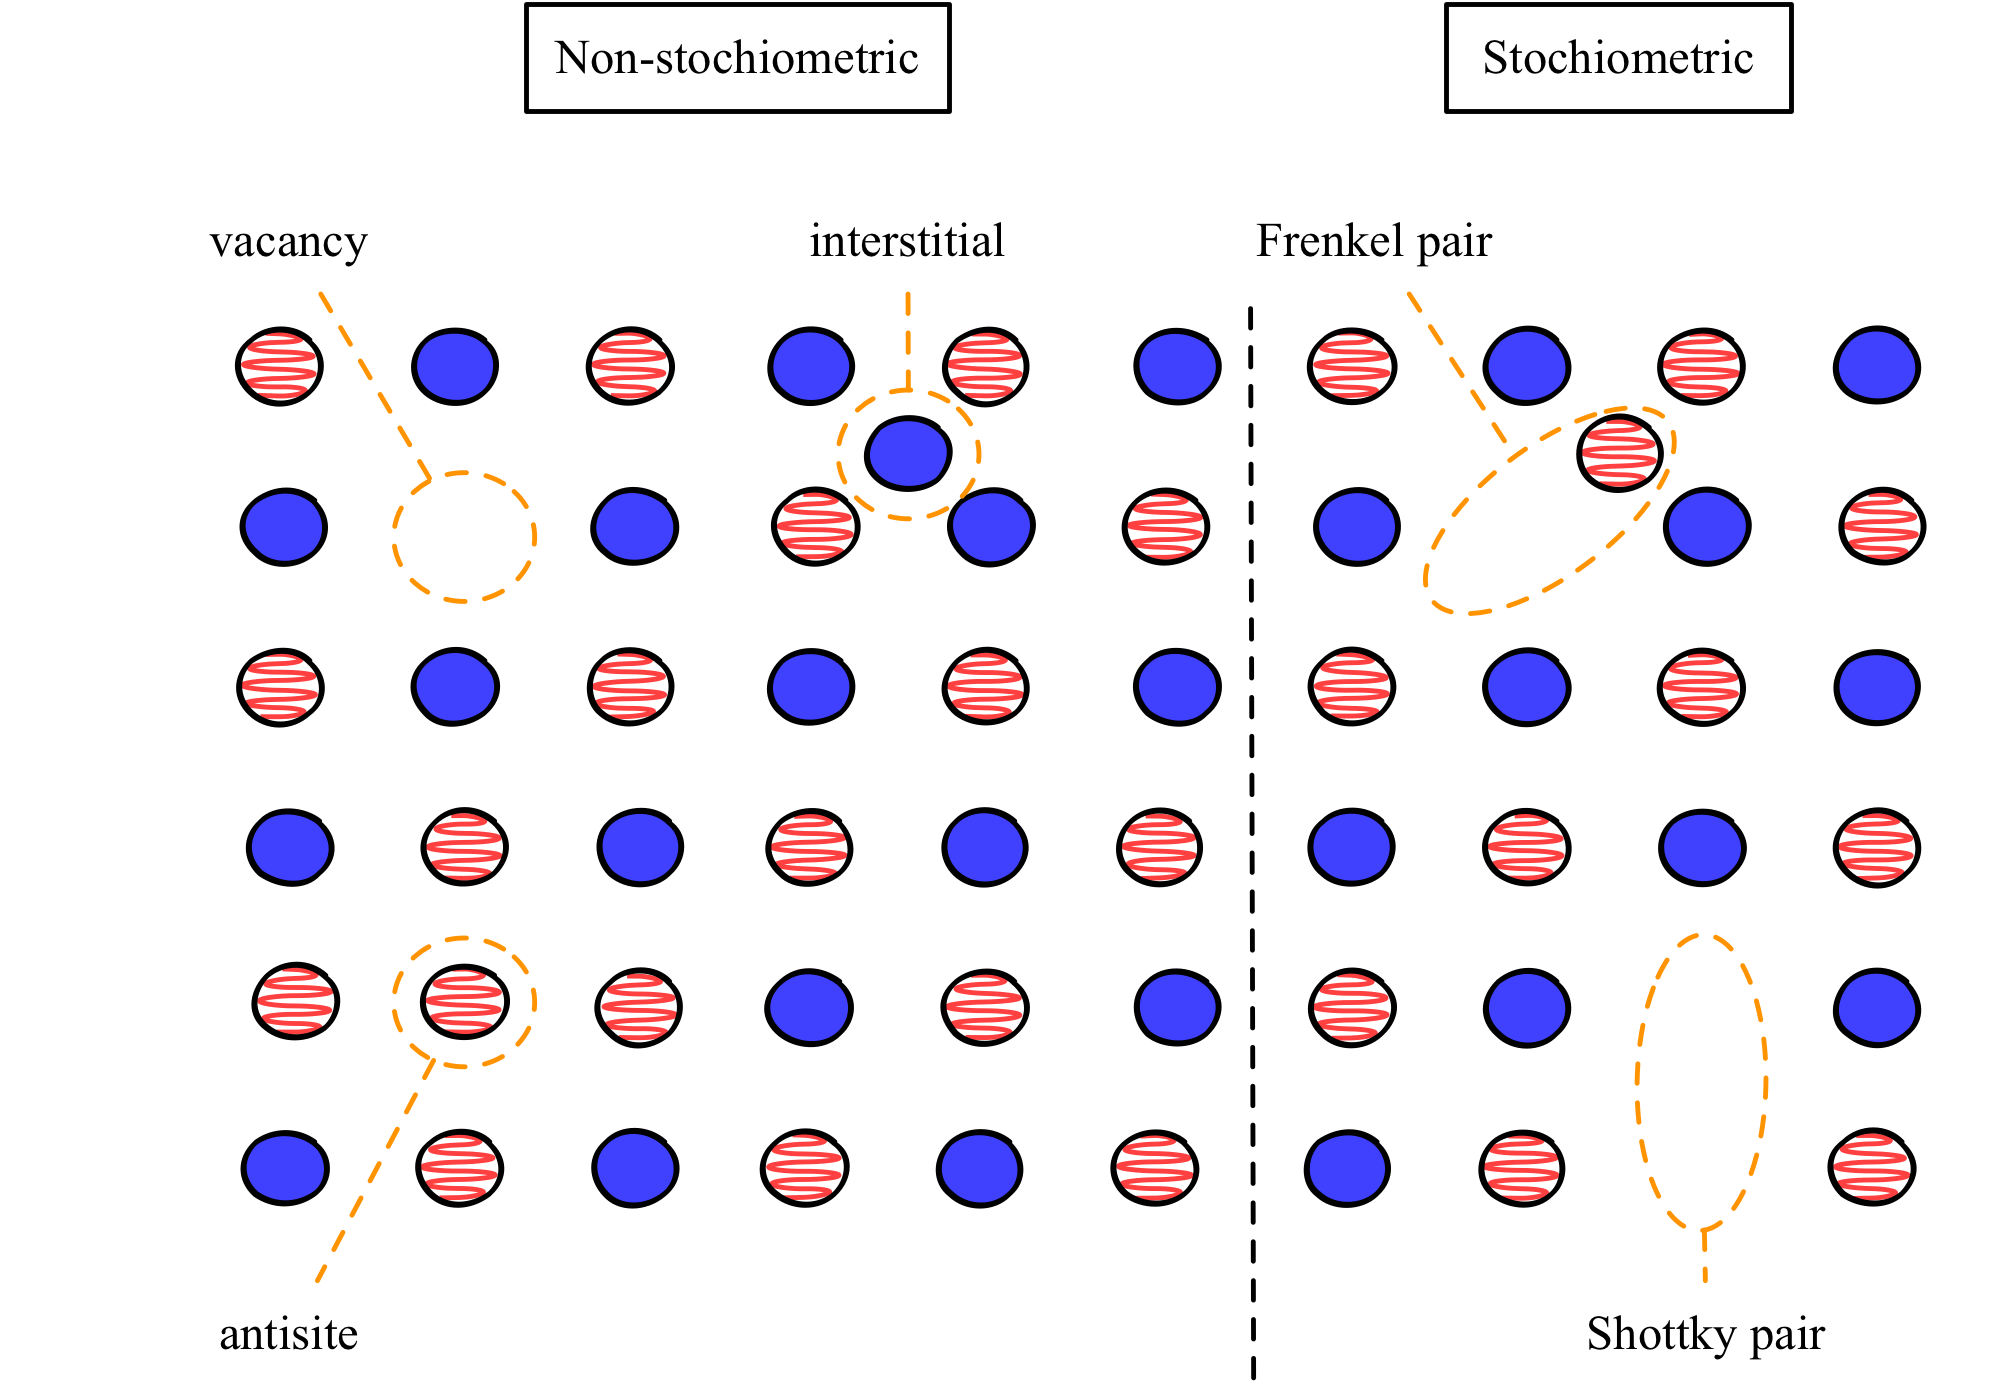
\includegraphics[resolution=450]{figures/ch3/classification.png}
  \caption[Classification of crystal point-defects]{A nearby pair of a vacancy and an interstitial is a Frenkel pair, whereas vacancies on both the anion and cation sub-lattices is a Shottky pair}
  \label{classification}
\end{figure}

The final classification is into electrically active and electrically benign defects. Whilst electrically benign defects exist only in one charge state, electrically active defects can take more than one charge state; for example, single acceptors exist in a neutral or negatively charged state and single donors exist in a neutral or positively charged states. Amphoteric defects can exist in a negatively charged or positively charged state.
% reference alkasukas https://www.osti.gov/pages/servlets/purl/1471061
% - may be able to say defect is there experimentally but another step to identify which it is. Admittance spectroscopy, DLTS. ESR (later chapter)
% emphasise that the concentration could be as low as one part in a milllion and wtill have an effect.
% - defect levels deend on temperature. DLTS assumes T-independant scattering cross sction, not accurate,

\subsection{The energetics of defect formation} \label{defectformation}

The equilibrium concentration of defects ($n$) at a fixed temperature and pressure is given by the density that minimizes the free energy.
\begin{equation} \label{defectconcentration}
    n = N_{sites} \exp \left(-\frac{\Delta G}{k_\mathrm{B} \mathrm{T}} \right),
\end{equation}
where $\Delta G$ is the Gibbs free energy of defect formation. The Gibbs free energy is approximated as the formation energy of the defect $\Delta E_f$ as this dominates over entropic contributions. The formation energy is given by
\begin{equation} \label{eqn_formation_energy}
E_f(q) = E_d(q) - E_b [-] \sum_i \mu_i n_i + q(\epsilon_\mathrm{VBM}+E_F) + E_{corr}
\end{equation}
where $E_d(q)$ is the total energy of the defect supercell and $E_b$ is the total energy of the perfect bulk. 
$E_{corr}$ is a correction energy that is only needed for charged defects, and is discussed further in the following section.
The remaining terms describe the energy needed to add or remove atoms and electrons.
$\mu_i$ is the chemical potential of the atom, and $n_i$ is the number that is added or removed.
The chemical potential can be adjusted to describe different growth conditions; if the growth conditions are rich for species $i$ then $\mu_i$ will be low.
$E_F$ is the Fermi level, referenced to the valence band maximum ($\epsilon_\mathrm{VBM}$).

The total energies can be calculated using DFT. Convergence criteria for calculations must be tight as, due to the exponential dependence of defect concentration on formation energy, small errors in the energy difference can lead to large errors in defect concentration.

The Fermi level is treated as a parameter, of which the defect formation energy is a linear function with a gradient equal to defect charge. This allows us to plot a graph of formation energy against Fermi level, as shown in Figure \ref{}. Charge transition levels mark the fermi energy at which two charge states have the same defect formation energy. Electrically active defects have at least one charge transition state in the band gap. 
The charge transition level is equivalent to thermal ionization energy, the energy needed to add or remove electron(s). % check this
% does not always need a charge transition level deep in the band gap. https://pubs.acs.org/doi/pdf/10.1021/acsenergylett.7b01313

\begin{figure}[h]
\centering
  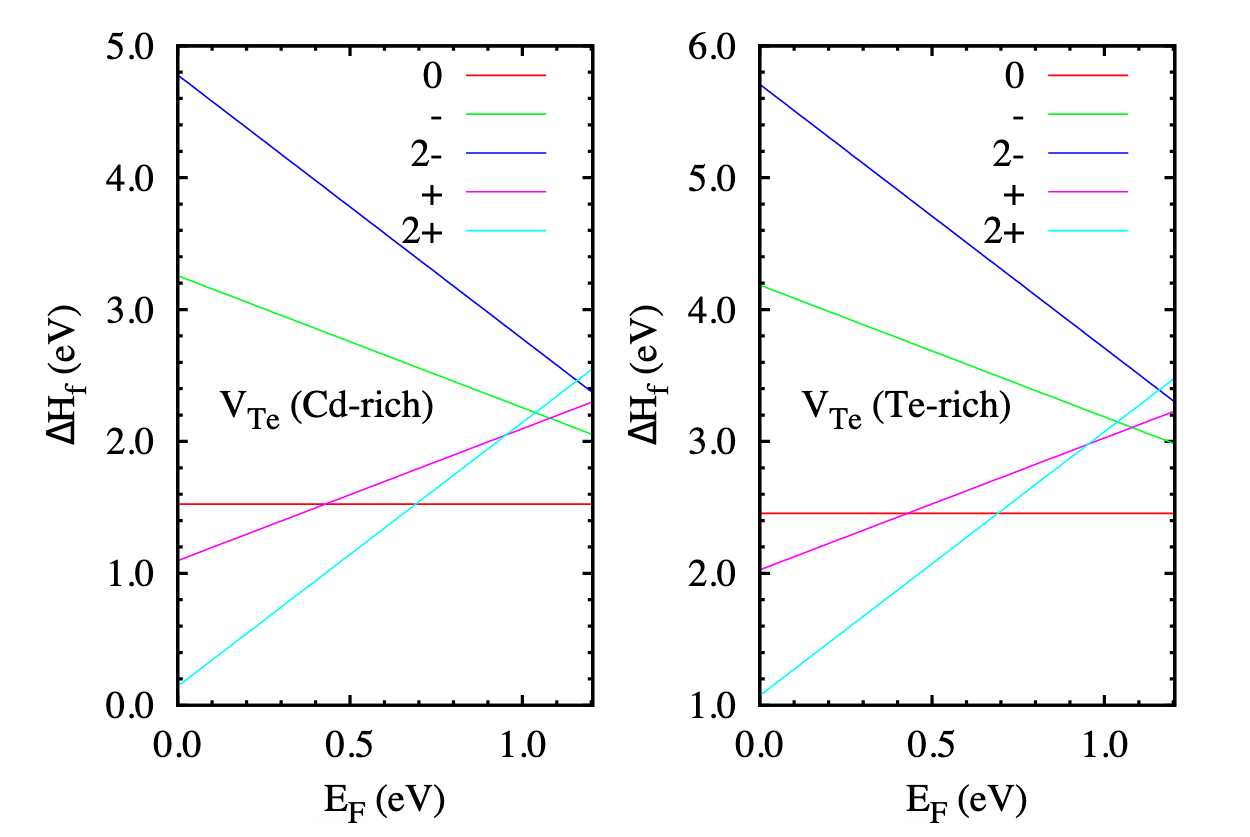
\includegraphics[resolution=450]{figures/ch3/defectenergetics.png}
  \caption[]{A nearby pair of a vacancy and an interstitial is a Frenkel pair, whereas vacancies on both the anion and cation sub-lattices is a Shottky pair}
  \label{defectenergetics}
\end{figure}

Defect levels deep in the band gap correspond to localised wavefunctions. Carrier capture to these defect states is often associated with a large lattice distortion. Shallow defect levels (within thermal energy $kT$ of the valence or conduction band) correspond to delocalised, hydrogenic-like defect wavefunctions. 
% - defect energies theoretical founsations - mott littleton (1938)  - a way to calculate E the defecct energy as knew the hopping rate expression, but didnt know E. only experimental input is dielectric constant.see special 1988 issue.
%  The other problem is that is dependant upon the chemical potential which is difficult to monitor.

% Point defects result in additional energy levels in the band gap with an associated defect wavefunction to which an electron is added or removed.
% defect level delocalised, electrical conductivity.EMT.
%or deep and localised wavefucntion. detrimental in the context of solar cells.

%The concentration of a point defect in a particular charge state can be controlled by tuning the Fermi level through doping. However there is a compensation mechanism, whereby defects form to compensate

% The concentration of point defects can be controlled by thermal treatment, irradiation or doping. 
% - Fermi level pinning (?) / defect concentration: Happens in TCO’s such as FTO. Above a certain concentration there are no more holes. This could happen when there are defect complexes which compensate each other.
% - This is a compensation mechanism. We try to adjust the fermi level of the system by introducing impurities. However above/below a certain energy level there is spontaneous formation of defects (defects which have a negative energy of formation). These defects compensate for the impurity and in this way the fermi level is pinned.

% - Calculable and observable table:
% Delta E : heat of formation / concentrations
% Defect ionisation – optical – instanataneour: PL, optical absorption / photoconductivity
% Defect ionisation , thermal, after relaxation: DLTS / thermally stimuated conductuvtiy
% Defect vibrational modes: IR/raman spectra and recombination rates

\subsection{The supercell method}

Defect concentrations as low as one part in one million can have an influence on device performance. 
One way to model point defects in the dilute limit, when defect-defect interactions are negligible, is to build a supercell from multiple unit cells (Figure \ref{}).
This supercell must be large enough so that there is no interaction between a defect and its periodic images.
This is the approach used in this work.
Although the supercell method captures localised defects well, it cannot capture the behaviour of delocalised (or band resonant) defects due to the enforced periodicty. 
%http://cmt.dur.ac.uk/sjc/thesis/thesis/node71.html


It is possible to remove the constraint of translational symmetry and use an embedded approach whereby a region around the defect is modelled using DFT and this is embedded in a region that is modelled classically.

% - The supercell method leads to some unphysical results for both electronic and vibrational properties. The defect will perturb the lattice. The SC method captures localised defect effects well – but the delocalised defects (possibly in the band) are not captured as there is an enforced periodicity. The only way around this is to use greens functions method (phonons) or QM/MM approach (electrons).
% vibrations of defects - link to final chapter

\subsubsection{Supercell corrections}
% this is from the joint JPhysChem defects review paper - if its published I will need to cite it!
% previous section - defect-defect interaction but there are also longer ranged coloumb interations
Point defects can be electrically charged, and are able to change charge state through the trapping and de-trapping of electrons and holes. 
The charge state of a defect can affect a number of defect properties including the preferred lattice position, surrounding lattice distortion, and the rates for diffusion, carrier capture, and carrier recombination.
However understanding the properties of charged defects is a challenge for DFT with periodic boundary conditions, due to the long range nature of the Coulomb interaction.
There are two issues to resolve. 
Firstly, charged defects are able to interact with their periodic images; 
Secondly, a homogeneous "jellium" background charge is introduced to ensure overall charge neutrality. This results in an unknown shift to the average electrostatic potential. 
These are finite-size effects, that only a very large, almost infinite, supercell would overcome as the Coulomb potential decays very slowly.
Such a supercell would certainly prove too costly, especially when higher levels of theory (for example, hybrid functionals) are required to calculate accurate total energies.

A number of correction schemes have been developed to deal with these issues; a brief historical overview is given below. These schemes are designed to be used as a post-processing step and provide a value for the $E_{corr}$ term in Eqn.\ref{eqn_formation_energy}. For a more complete description of these issues we refer the reader to the existing literature.\cite{durrant2018,Vinichenko2017}

The Leslie Gillan correction\cite{Leslie1985} models the defect charge $q$ as a point charge interacting with it's periodic images through an isotropic dielectric medium. 
This correction takes a simple analytic form that depends on the charge state  $q$, static dielectric constant $\epsilon$, separation between images $L$ and the Madelung constant $\alpha_m$, which is determined by the lattice geometry.
The Markov-Payne correction extends the Leslie Gillan correction by including an additional term which accounts for the delocalised part of the defect charge. 
\begin{equation}
    E^\mathrm{MP} = \frac{q^2\alpha_{m}}{2\epsilon L} [+ qQL^{-3}]
\end{equation}

The challenge of this approach is in calculating the quadrupole moment $Q$. 
The Lany-Zunger correction\cite{Lany2009} combines the Markov-Payne correction, including an approach for calculating $Q$, with a potential alignment procedure to correct for the shift in electrostatic potential. 
The Freysholdt, Neugebauer and van de Walle (FNV) method\cite{Freysoldt2009} models the defect charge as a localised gaussian distribution. 
The difference between the electrostatic potential of the charged defect supercell and the electrostatic potential of the perfect bulk supercell, calculated far from the defect, is aligned with the defect model potential. 
Kumagai and Oba have extended to FNV method by using atomic site potentials combined with a point charge model for an anisotropic medium.\cite{Kumagai2014} 

The schemes discussed were initially developed for use with three-dimensional materials. 
Recent work has extended these methods to two-dimensional\cite{Freysoldt2018,Komsa2013} and one-dimensional\cite{Kim2014} materials.
We note that there is still no standardised approach to defect charge corrections, 
which can lead to a spread in calculated defect formation energies in the literature, and predicted defect densities which differ by orders of magnitude.
Two widely used approaches in the recent literature are the FNV method, and the extension to this provided by Kumagai and Oba.
Both schemes are implemented in the \texttt{sxdefectalign}, as outlined in the following section.
Developing an efficient scheme which can account for microscopic effects and anisotropy is an active area of research.\cite{durrant2018,Vinichenko2017}
% - for a really good explanation see Suzys group talk (Monday the 10th september 2018) and https://aip.scitation.org/doi/10.1063/1.5029818 which it was based upon.
%what are the corections used in this work?


\section{Calculating the properties of vibrations in crystals} \label{sec:latticedynamics}
%cite defect and defect processes in nonmetallic solids
%cite Dove Lattice dynamics

Heisenberg's uncertainty principle, a central principle of quantum mechanics, states that we cannot know both the position and momentum of a particle exactly. Thus the static lattice model used so far is not true for real material; even at $T=0\,\textrm{K}$ there is zero point motion. As temperature increases, this motion increases in amplitude.

Understanding the vibrations of crystals is key to understanding a range of physical phenomena. The motion of the atoms have an associated vibrational energy, and this determines crystal stability as a function of temperature via the Gibbs free energy:
\begin{equation}
G = E_0+E_\textrm{vib}+PV-TS
\end{equation}
where $E_0$ is the ground state energy as calculated using DFT and $E_\textrm{vib}$ is the vibrational contribution to internal enery.
Atomic motion also influences electrical and optical crystal properties; this can be seen experimentally in the homogeneous broadening of photoluminescence linewidths with temperature.%cite https://journals.aps.org/pr/abstract/10.1103/PhysRev.128.1726
Other material properties which are only accessible via lattice dynamics include: heat capacity, thermal conductivity, elasticity, thermal expansion coefficients, electron-phonon coupling strengths and static polarization.

For atomic motion at small amplitudes around the potential energy minimum it is common to use the harmonic approximation, where the atom moves as if it is connected by a spring to its neighbouring atoms (Figure \ref{harmonicregime}). This is discussed in Section \ref{harmonicapprox}. At larger vibration amplitudes, and to understand processes related to the creation and annihilation of phonons, we must consider anharmonic motion, and this is considered in Section \ref{anharmonicapprox}.

These motions are determined by the force on each atom. For simple systems, for example a one-dimensional diatomic chain, we can calculate atomic position as a function of time analytically. Otherwise methods such as DFT can be used to build a force constant matrix which, after some post-processing steps, gives the eigenvectors (direction) and frequencies of motion. This is discussed in Section \ref{finitedisplacement}. As in the previous sections of this chapter, we use the Born-Oppenheimer approximation and assume that the equilibrium positions in a crystal are the minima of the potential energy surface when the electron and nuclear motion are decoupled.

\begin{figure}[h]
\centering
  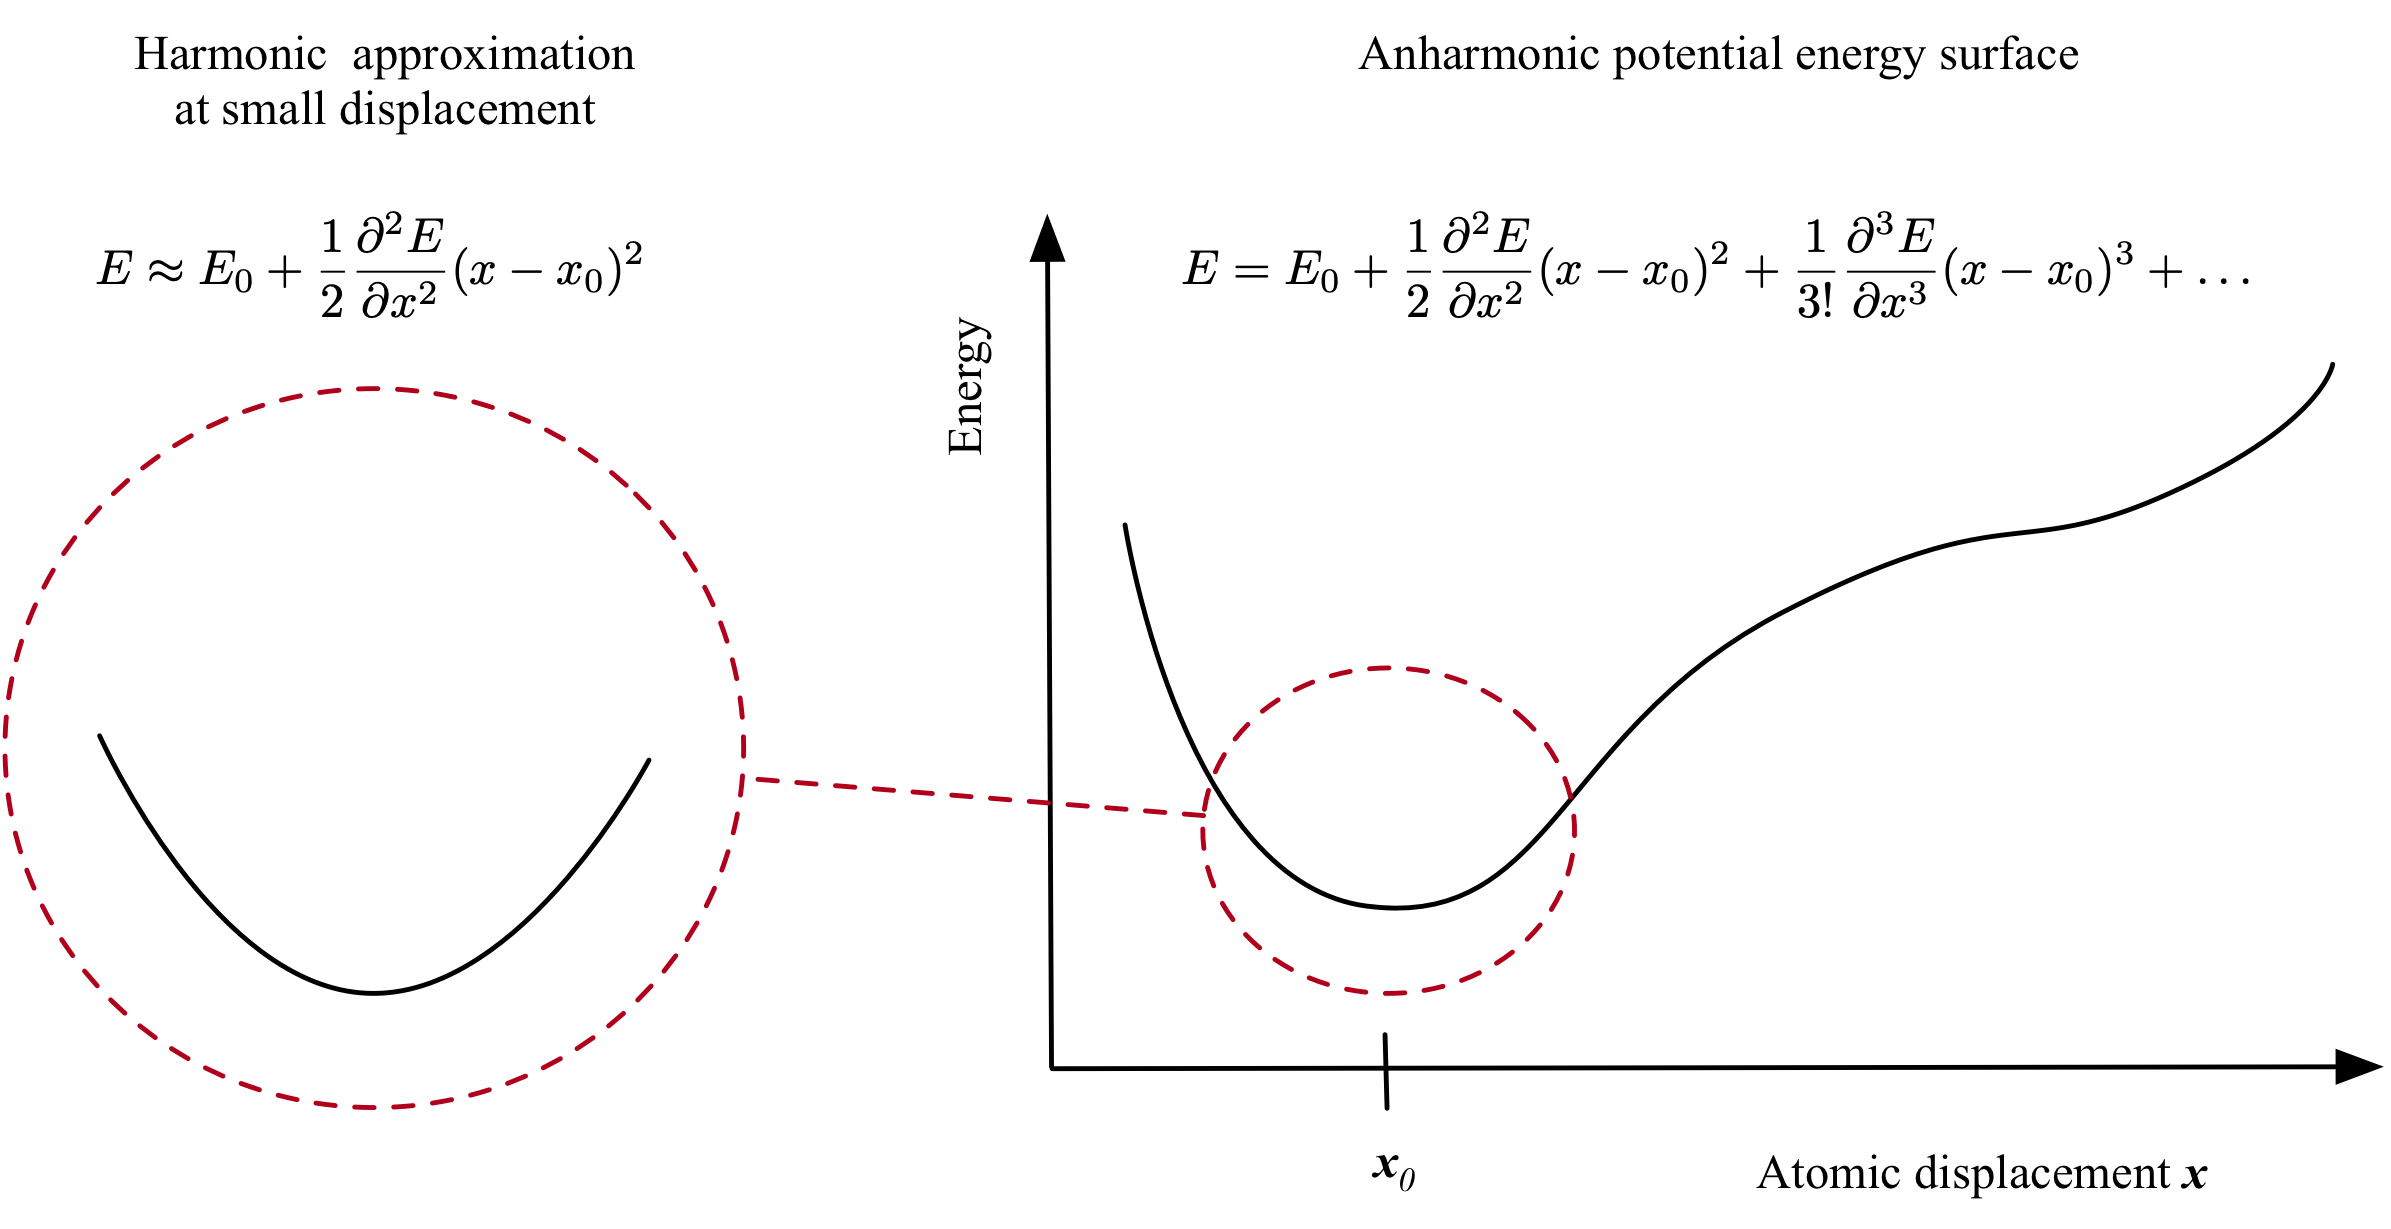
\includegraphics[resolution=450]{figures/ch3/harmonicregime.png}
  \caption[]{}
  \label{harmonicregime}
\end{figure}



%important to understand crstal stabilit as the vibrational energy and entropy enter the Gibbs free energy
% - Partition function ---> bridge function kTlnZ (bridges micro and macro thermodyamics) to get helmholtz free energy. need vibrations to get temperature dependant energy and stability as a function of temperature.

% We know this affects electrical and optical properties – look at the peak shift in energy and peak broadening ith temperature.
% % - model for vibrations (harmonic approximation) ---> vib freq and displacement patterns (vibrational spectra) and from that IR/raman, free energies (T) - phase change. all stuff you couldnt get with standard electronic structure
% thermodynamics requires phonons, (helmholtz free energy)


% - What information can we get from phonons? 
% Thermodynamic quantities at low temperature: heat capacity, entropy, free energy, zero-point,
% Phase transitions from the Gibbs free energy,
% Conductivity,
% Infromation about lattice instabilities in the form of imaginary frequencies,
% Elastic tensor from the q to zero limit of phonon dispersion,
% Thermal expansion coefficient,
% Temperature dependence of the band gap,
% Electron phonon coupling strengths,
% Static polarization

% - Experimental evidence:
% Measured directly with inelastic scattering,
% IR and Raman spectroscopy


% - For small amplitudes we consider a simple harmonic motion. phonon modes are uncoupled and have infinite lifetime.
% - At larger amplitudes we must consider anharmonic motion. phonons can be created and destroyed, have a lifetime and give access to new properties.
% - Extent of Anharmonicity depends upon how much of the potential energy space you are exploring ((tie in with perturbative and non-perturbative regime skethc). At low T you may be exploring harmonic potentil like minima, at High T you may be beyond this minima
% - Adiabatic approximation: Can thin of electronic wavefunction for eignstate of nuclei fixed in position.


% - The motions are determined by atomic forces. For a 1D system with a single mass or with two masses (lattice with basis) we can solve analytically. Otherwise these can be determined through DFT calculations (Hellman Feynmann theorem), producing a force constant matrix. 

% - Table with the approximation and the properties you can get and codes which implement....
% - quasi-harmonic:properties as a function of volume.helmholtz as function of temeparture  - at some point it is favourable to have a different volume . Free energy as function volume for several tempatures and the fit an equation of state. 
% - Then you can get the bulk modulus, heat capacity constant pressure, gibbs free, gruneisan, volumetric thermal expansion.use to get properties at finite T - use the structure which minimises for a particular temp.
% - Thermal expansion coefficients, system anharmonicity (e.g. modal grun parameters) and the temperature-dependence of other properties can be calculated in the quasi-harmonic approximation (QHA). 
% Here the lattice dynamics is harmonic at a given temperature; however, the cell volume is scaled by thermal expansion to give the first-order contribution of finite temperature effects. 
% 2: frequency and eigenvectors
% 3: phonon linewidths / spectral lifetimes
% 4: anharmonic frequency shifts
% https://thelostelectron.wordpress.com/

\subsection{The harmonic approximation} \ref{harmonicapprox}

If displacements from equilibrium are small, the total energy can be Taylor expanded in the form 
\begin{align} \label{taylorexpansion}
E&=\textrm{kinetic energy}+\textrm{potential energy}
&=\sum_i\frac{1}{2}M\dot{x}_i^2+\sum_{ij}\frac{1}{2}\textbf{x}_i\cdot\textbf{A}_{ij}\cdot\textbf{x}_j+\textrm{higher-order terms}.
\end{align}

The structure is relaxed and forces are equal to zero so that there is no term linear in $\textbf{x}$. The harmonic approximation ignores the higher order terms in Equation \ref{taylorexpansion}. For these harmonic systems there exists a basis set so that $\textbf{A}_{ij}$ is diagonal and the oscillators are independant of one another:
\begin{align} \label{independentoscillators}
&=\sum_i\frac{1}{2}MQ_i^2+\sum_{i}\frac{1}{2}\textbf{A}_{ij}\cdot\textbf{x}_j+\textrm{higher-order terms}.
\end{align}
The general solution to this system of equations for an $N$-atom unit cell in three dimensions is a superposition of $3N$ normal modes of vibration, each with its own frequency and eigenvector.
To calculate the normal modes (phonons) we start Newton's second law, $F=ma$. For crystalline solids we take advantage of symmetry and seek normal modes that for a chosen wavevector $k$ are a linear combination of a relative displacement within the unit cell $\textbf{u}_0(i,\textbf{k})$, a phase that depends on the unit cell $\textrm{exp}(i\textbf{k}\cdot\textbf{R}_I)$, and an oscillation in time $exp(i\omega(\textbf{k})t)$
\begin{equation} \label{normalmodes}
\textbf{u}_0(i,\textbf{k})\textrm{exp}(i\textbf{k}\cdot\textbf{R}_I)exp(i\omega(\textbf{k})t)
\end{equation}
If we seek displacements of this form, Newton's second law has consistent solutions only if the secular equation is satisfied:
\begin{equation}
\textrm{Det}|\sum_J A_{\alpha}{\beta}(iI,jJ)exp(i\textbf{k}\cdot\textbf{R}_J)-M_i\delta_{ij}\omega^2(\textbf{k})|=0
\end{equation}
where the first term in the determinent is called the dynamical matrix which is built from the force constant matrix $A_{\alpha\beta}$:
\begin{equation}
\textbf{A} = 
\begin{pmatrix} 
\frac{\delta^2E}{\delta x_1^2} &\frac{\delta^2E}{\delta x_1 \delta x_2} & \cdots & \frac{\delta^2E}{\delta x_1 \delta x_n}\\
\frac{\delta^2E}{\delta x_2 \delta x_1}&\frac{\delta^2E}{\delta x_2^2} & \cdots & \frac{\delta^2E}{\delta x_2 \delta x_n}\\
\vdots & \vdots & \ddots & \vdots \\
\frac{\delta^2E}{\delta x_n \delta x_1}&\frac{\delta^2E}{\delta x_n \delta x_2} & \cdots & \frac{\delta^2E}{\delta x_n^2}\\
\end{pmatrix}
\end{equation}

The normal mode frequencies are the roots of Equation \ref{normalmodes} and can be found through matrix diagonalisation. Plotting the frequency $\omega$ against wavevector $k$ gives a bandstructure plot with periodicity $\frac{2\pi}{a}$, similar to that in Section \ref{}.   %check that a is correct for lattice length 

The discussion so far has only used classical mechanics. To introduce quantum effects we recognise that the harmonic lattice vibrations will be analogous to a quantum simple harmonic oscillator and so will be restricted to certain energy values $E_n = (n+\frac{1}{2}\hbar\omega)$.
Once the phonon eigenvectors and frequencies are found we have access to the Gibbs free energy and heat capacity.

% The phonons of energy hbar omega have exact energy so cannot be localised in space: formed of delocalised plane waves
% But can construct localized packet using modes of different fequency. Can then treat phonons as localised particles. E = hbar omega. K is the crystal momentum .
% Phonons are bosons, not conserved. They can be created and destroyed. 

% once got eigencevtors nad freuencies have access to toher props via partition function

\subsection{Anharmonicity} \ref{anharmonicapprox}

Anharmonic atomic motion is considered when the higher order terms in Equation \ref{taylorexpansion} are included.
When the third order term is included it is possible to consider phonon-phonon scattering which, due to the conservation of energy and momentum, is a three particle process.
The phonon-phonon scattering rate gives the thermal conductivity of a material :

%Calculate a third order force-constant matrix. Can calculate phonon-phonon coupling terms and low thermal conductivity. Number of channels and strneght of coupling. GaAs vs MAPI. Discussed in paper. Required 41,544 displacements. 96 atoms
%Expresion for thermal conductivtiy, product of heat capacity, group velocity and mean free path.
% - Phonons from DFPT: http://journals.aps.org/rmp/pdf/10.1103/RevModPhys.73.515 - a good outline of the theory implemented in phono3py.
% - The thermal conductivity as calculated in phono3py depends upon the single mode relaxation time approximation (see togo’s theory paper on this). This is where the lifetime as of a single mode as calculated in phono3py is set as the relaxation time in the linearised boltzmann transport equation.
% Under this assumption the thermal conductivity is then a summation over the product of heat capacity, mode velocity and relaxation time, which all come out of phono3py
% - emphasise the cost required
% -  can reduce the cst by just considering the phase space (broido talk, laptop notes)



Anharmonic motion is also important in materials near a phase transition. % - anharmonicity schematic under visuals: Si, PbTe, SrTiO3% - Anharmonicity also needs to be considered according to material (schematic here)
% for some vobrations compression and extension will not be equal curvature. talk about % - harmonic approximation expects the energy to increase as you push along the mode.imaginary frequency because $w^2$ is negative.
% - dynamic stability if all positive
%- mechanism for some phase transitions is where phonon mode becomes imaginary at a transition temperature



% - Anharmonicity most important when under high pressure or high temperature (bouchert) which is often the case for geophysical applications.



% - Navaneeth : assessing how higher order anharmonicity can aggect htermal conductivity. In Diamond the 4 phonon phase space is 10x that of 3-phonon. In Bas it is 100X that of 3-phonon phase space. We must then also consider the scattering strength (can only consider the scattering rate of those with a large phase space). The size of these phase spaces are huge. For example, Bas which is in the zincbelnde structure has 6 polarisations. If each done explicitly there would be $9x10^ 3$-phonon calculations, for 4-phonon processes there would be $2x10^12$!!!  So instead temperature-dependent ensembles are used (where all atoms are moved at the same time, calculated from explicit 2nd order force constant calculation) and then used to fit 3rd and 4th order force constants to.



\begin{figure}[h]
\centering
  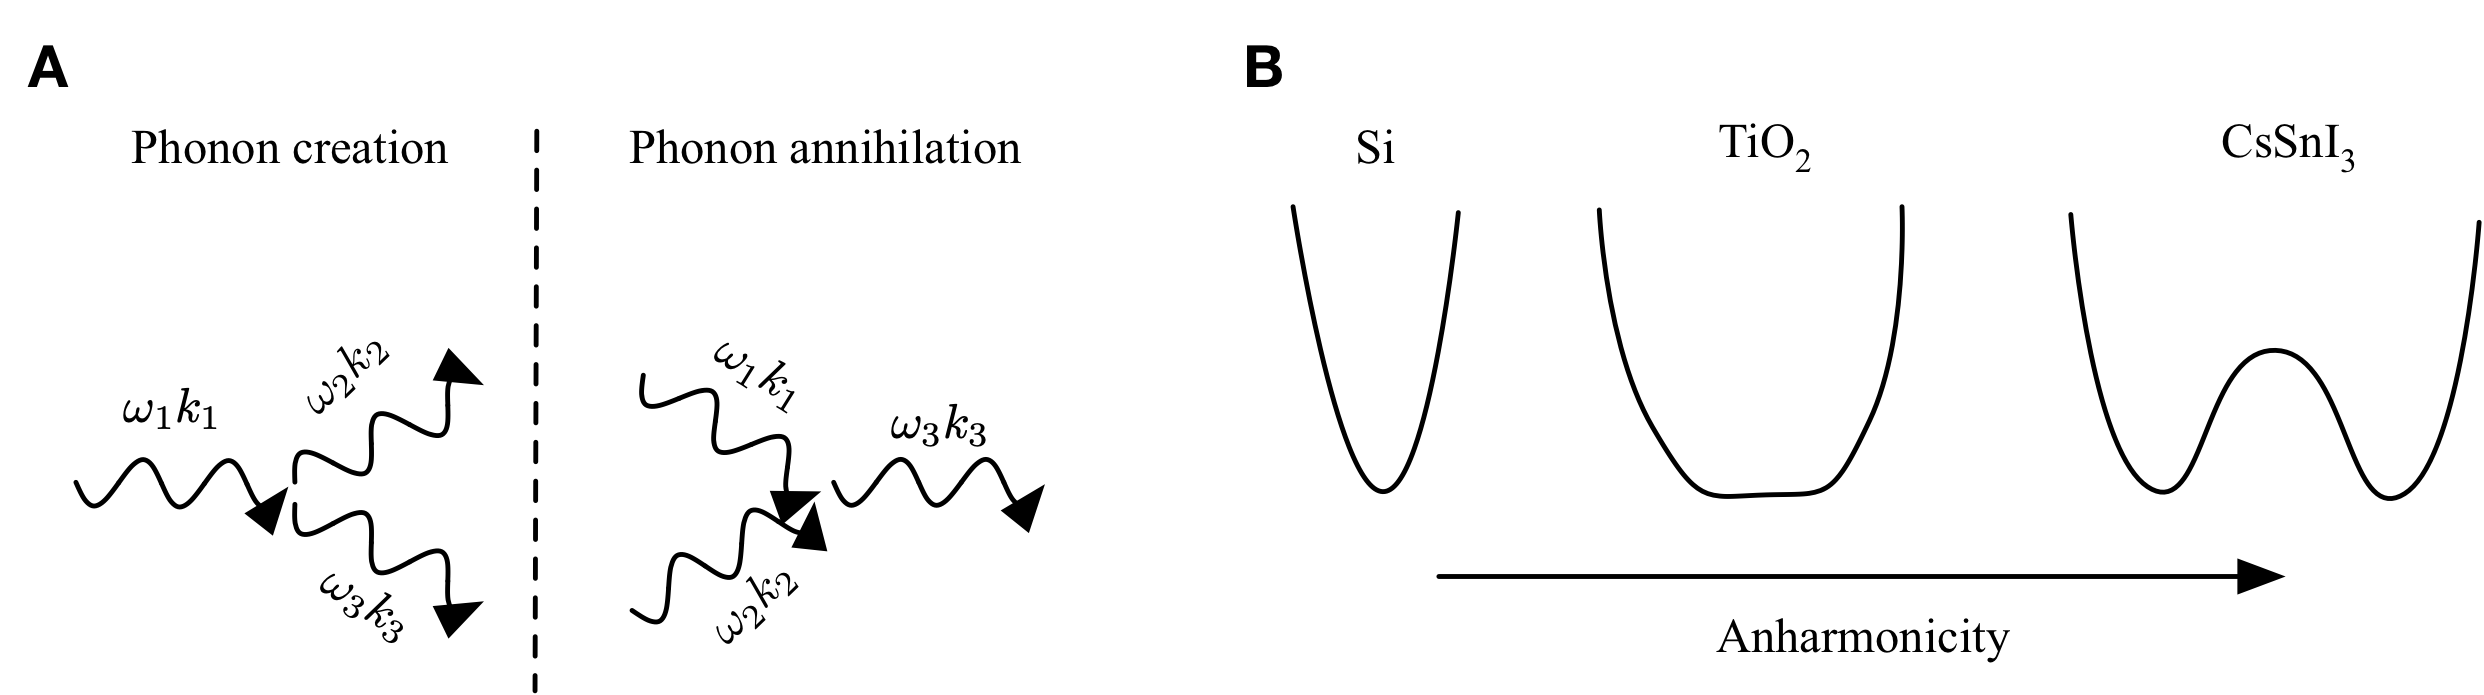
\includegraphics[resolution=450]{figures/ch3/anharmonicity.png}
  \caption[]{}
  \label{harmonicregime}
\end{figure}  %include phonon-phonon scattering schematic? the third regime where important is given in the other figure, at high temperature



\subsection{The finite displacement method} \ref{finitedisplacement}

% - Note that the  eigenvalue equation for the dynamical matrix is gotten from fourier transform
% Of the taylor expansion of the crystal potential.
% - force constant matrix . then construct dynamical matrix - -> wavevector. then diagonalise - the eigenvectors and eigenvalues. do a schematic for this process. then two ways to get to the dynamical matrix.

% - There are a multitude of ways to calculate these force constants: explicitly (finite difference, DFPT for 3rd or 4th orders), empirical potentials (TDEP), compressive sensing lattice dynamics or beyond perturbation (AIMD,PIMD,SCAILD, variational methodslike SSCHA developed by Ion Errea).
% - perturbation theory- dynamical matrix directly. no supercell and more accurate but constrained which functionals and pseudopotentials you need.

% schematic of workflow: input structure, create displacements, calculate forces, calculate dynamical matrix, diagonalise

\begin{figure}[h]
\centering
  \includegraphics[resolution=450]{figures/ch3/phononworkflow.png}
  \caption[]{}
  \label{harmonicregime}
\end{figure}

% in this work the finite displacement approach is used as implemented in...
% For derivatives we exploit the hellman-feynam theorem and use finite differences % - Force constant via finite displacement - displace small and calculate force. Simple, general and can split into small jobs (parallelise). 
% AKA "supercell","direct" or "frozen phonon" 
% - phonons can have a wavelength longer than the size of the supercell - need to capture the longer wavelength. but need supercells. use phonopy. Maximum is 6N displacements but this is seriously reduced by symmetry. (spglib)
% - Need good relaxation: don't skimp on the forces, cutoff or k-points.
% - PBEsol for reproducing lattice constants and phonons (Jonathan 2015 J.Chem. Phys)

% - See Jonathans talks

\section{Summary}

%: LW - could we add here that solid state physics of crystalline materials is not really built for defects as they assume perfect translational symmetry, which the defects break ---> which makes modelling defects a continuing challenge for theory and simulation (as we are working "against" the fundamental assumptions of the framework).
% - defects are demainding and computational expensive .n To avoid computationally expensive defect calculations descriptors have been built on the idea of ‘defect tolerant’ materials: http://pubs.acs.org/doi/pdf/10.1021/acs.nanolett.5b04513
% in fact I combine defect and phonon calculations in final chapter


